% !TEX TS-program = pdflatex
% !TEX encoding = UTF-8 Unicode

% This is a simple template for a LaTeX document using the "article" class.
% See "book", "report", "letter" for other types of document.

\documentclass[11pt]{article} % use larger type; default would be 10pt

%\usepackage[utf8]{inputenc} % set input encoding (not needed with XeLaTeX)

%%% Examples of Article customizations
% These packages are optional, depending whether you want the features they provide.
% See the LaTeX Companion or other references for full information.

%%% PAGE DIMENSIONS

\usepackage{geometry} % to change the page dimensions
\geometry{a4paper} % or letterpaper (US) or a5paper or....
%\geometry{margins=2in} % for example, change the margins to 2 inches all round
% \geometry{landscape} % set up the page for landscape
%   read geometry.pdf for detailed page layout information
\usepackage{fullpage}
%\usepackage[top=tlength, bottom=blength, left=llength, right=rlength]{geometry}
%Edit individual page dimension variables described above, using the \addtolength and \setlength commands. For instance,
%\oddsidemargin=-1cm
%\setlength{\textwidth}{6.5in}
%\addtolength{\voffset}{-5pt}

\usepackage{graphicx} % support the \includegraphics command and options

% \usepackage[parfill]{parskip} % Activate to begin paragraphs with an empty line rather than an indent

%%% PACKAGES
\usepackage{booktabs} % for much better looking tables
\usepackage{array} % for better arrays (eg matrices) in maths
\usepackage{paralist} % very flexible & customisable lists (eg. enumerate/itemize, etc.)
\usepackage{verbatim} % adds environment for commenting out blocks of text & for better verbatim
\usepackage{subfig} % make it possible to include more than one captioned figure/table in a single float
\usepackage{cite}
\usepackage{graphicx}
\usepackage{hyperref, amsmath, mathrsfs, bm}

\usepackage{url}
\renewcommand{\thesubfigure}{}
% justifying
\usepackage{ragged2e}


\graphicspath{{./}{./graphs/}{./../graphs/}{./../../DataFusion/graphs/}{./../../DataFusion_Kconditions/graphs/}}


\usepackage{amssymb,amsmath,amsthm,amscd}

\usepackage[mathscr]{eucal}
%\usepackage[dvips]{graphicx}
%\usepackage{pstricks,pst-grad,pst-plot,pst-node}


%\usepackage{pgf}



%\newpsobject{showgrid}{psgrid}{subgriddiv=1,griddots=2,gridlabels=6pt}
\renewcommand{\raggedright}{\leftskip=0pt \rightskip=0pt plus 0cm}
% argmin
\DeclareMathOperator*{\argmin}{arg\,min}

\newcommand{\myred}{\color{red}}
\newcommand{\mygreen}{\color{green!50!black}}
\newcommand{\myblue}{\color{blue}}

\newcommand{\mcX}{\mathcal{X}}
\newcommand{\mcY}{\mathcal{Y}}
\newcommand{\mcG}{\mathcal{G}}
\newcommand{\mcF}{\mathcal{F}}


%\usepackage[tiling]{pst-fill}
\usepackage{epsfig}
\usepackage{graphicx}
\usepackage[usenames,dvipsnames]{color}

\usepackage{Sweave}
\usepackage{tikz}
\usepackage{pgf}

%%% HEADERS & FOOTERS
\usepackage{fancyhdr} % This should be set AFTER setting up the page geometry
\pagestyle{fancy} % options: empty , plain , fancy
\renewcommand{\headrulewidth}{0pt} % customise the layout...
\lhead{}\chead{}\rhead{}
\lfoot{}\cfoot{\thepage}\rfoot{}

%%% SECTION TITLE APPEARANCE
%\usepackage{sectsty}
%\allsectionsfont{\sffamily\mdseries\upshape} % (See the fntguide.pdf for font help)
% (This matches ConTeXt defaults)

%%% ToC (table of contents) APPEARANCE
\usepackage[nottoc,notlof,notlot]{tocbibind} % Put the bibliography in the ToC
\usepackage[titles,subfigure]{tocloft} % Alter the style of the Table of Contents
\renewcommand{\cftsecfont}{\rmfamily\mdseries\upshape}
\renewcommand{\cftsecpagefont}{\rmfamily\mdseries\upshape} % No bold!

\newtheorem{thm}{Theorem}
\newtheorem{cor}{Corollary}
\newtheorem{lem}{Lemma}





%%% END Article customizations

%%% The "real" document content comes below...

\title{Optimal Weighting for Joint Optimization of Fidelity and Commensurability in Tests of Matchedness}


%input affiliations


\author{Sancar Adali\thanks{Johns Hopkins University,
Department of Applied Mathematics and Statistics,
100 Whitehead Hall,
3400 North Charles Street,
Baltimore, MD 21218-2682} \and Carey E. Priebe\thanks{Johns Hopkins University,
Department of Applied Mathematics and Statistics,
100 Whitehead Hall,
3400 North Charles Street,
Baltimore, MD 21218-2682}
}
 

% \email{sadali1@jhu.edu}   %optional

% \email{cep@jhu.edu}   %optional
\date {August 1, 2011}% Activate to display a given date or no date (if empty),
         % otherwise the current date is printed 

\begin{document}
\maketitle
\abstract{For matched data from disparate sources (objects observed under different conditions), optimality of information fusion must be defined with respect to the inference task at hand. Defining the task as matched/unmatched hypothesis testing for dissimilarity observations, the forthcoming Manifold Matching paper by Priebe et al.~\cite{JOFC} presents an embedding method based on joint optimization of fidelity (preservation of within-condition dissimilarities between observations of an object) and commensurability (preservation of between-condition dissimilarities between observations) . We investigate the tradeoff between fidelity and commensurability by varying weights in weighted embedding of an omnibus dissimilarity matrix. Optimal (defined with respect to the power of the test) weights for the optimization correspond to an optimal compromise between fidelity and commensurability. The two extremes of this tradeoff are commensurability optimization prioritized over fidelity optimization and vice versa. Results indicate optimal weights are different than equal weights for commensurability and fidelity and our weighted embedding scheme provides significant improvements in test power.
}




\section{Introduction}

 It is a challenge  to do a tractable analysis on data from disparate sources of data(such as multiple sensors). The multitude  of sensors technology and large numbers of sensors both are  sources of difficulty and hold promise for efficient inference.
 The typical multiple sensor setting is visualized in ~\ref{fig:fig1}.

\begin{figure}
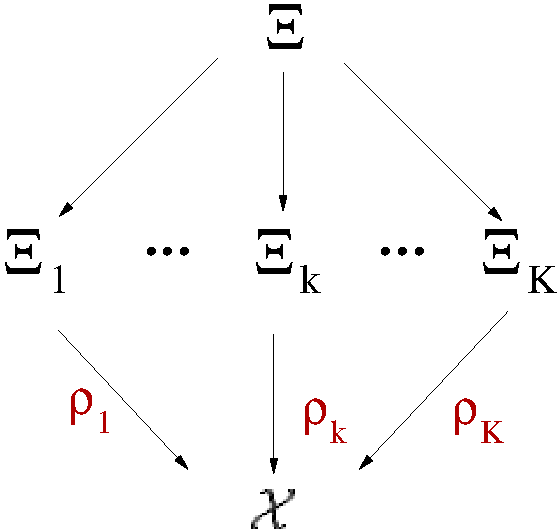
\includegraphics[scale=0.35]{gen-model-orig-proj.pdf}
\caption{Multiple Sensor setting}
\label{fig:fig1}
\end{figure}


We assume some objects lie in some "object`` space $\Xi$, and each sensor has another "view`` of the objects. The measurements recorded by the $i^{th}$ sensor lie in some "measurement space`` $\Xi_i$. The usual approach in pattern recognition is to use feature extractors on the spaces to get a feature representation in Euclidean space and use classical pattern recognition tools to carry out the exploitation task. The alternative approach is to acquire dissimilarities between the group of objects, and use the dissimilarities to either find an embedding in a low-dimensional Euclidean space where classic statistical tools are available for inference or use dissimilarity-based versions of pattern recognition tools~\cite{duin2005dissimilarity}. We will follow the embedding approach in a  low-dimensional Euclidean space where small number of dimensions allow us to avoid "curse of dimensionality``. We will require the embeddings of dissimilarities from  different conditions to be "commensurate`` so that sensor measurements can be compared or jointly used in inference. This is accomplished by maps $\rho_k,k=1,\ldots,K$ from measurement spaces $\Xi_k$ to a low-dimensional commensurate space $\mathcal{X}$ visualized in~\ref{fig:fig1}. Learning these maps from data is  an important portion of our approach.

There are quite  a few real life cases, where the data is acquired or available exclusively in dissimilarity representation instead of feature representation~\cite{CMDS,borg+groenen:1997,duin2005dissimilarity}.
 Multidimensional scaling is the processing step used to find the feature representation equivalent of this kind of data, so that  statistial machine learning methods can be applied to the data. A specific variant of MDS will be used to get an embedding in  Euclidean Space. Multidimensional scaling computes a configuration of points that has interpoint distances as close as possible to the dissimilarities in dissimilarity representation. Different criterion functions can be used to measure how close the distances are  to the given dissimilarities, the optimization of which leads to different embedded configurations. Among these, we seek configurations that have  the merit of  as close as possible to (in some sense) optimal in terms of the exploitation task we are interested in. In this paper, hypothesis testing is our exploitation task, and  by "optimal'' we mean the one that leads to the  test with  the highest power. Consider the weighted raw-stress function:
\begin{equation}
\sigma_{W}(X)=\sum_{1\leq s\leq n;1\leq t\leq n} {w_{st}(d_{st}(X)-\delta_{st})^2  }\label{raw-stress}
\end{equation}
 for an  $n \times p$ configuration matrix ($n$ points in $p$ dimensions)  $X$  where $d_{st}(X)$ is the Euclidean distance between $s^{th}$ and $t^{th}$ rows of $X$ and $w_{st}$ is the weight for $st^{th}$  squared difference.  We will refer to the $n \times n$  matrix representation of the weights and Euclidean distance as $W$ and $D(X)$, respectively. This   criterion function which will be minimized for embedding configurations is appropriate for our purpose of finding a tradeoff between two different criteria (namely the preservation of fidelity and commensurability).




Let us state the dissimilarity-representation version of a hypothesis testing problem:\\
$n$ different objects/instances are measured/judged under $K$ different conditions with (possibly notional) measurements $x_{ik}$ indexed by object and condition. Each of the measurements $x_{ik}$ lies in  the corresponding space $\Xi_k$. 
\[  \begin{array}{cccc}
        & \Xi_1 & \cdots & \Xi_K\\
        Object ~ 1 & \bm{x}_{11} & \sim \cdots \sim & \bm{x}_{1K} \\
        \vdots & \vdots & \vdots & \vdots \\
        %\text{Object} ~ i & \bm{x}_{i1} & \sim \cdots \sim & \bm{x}_{iK} \\
        %\vdots & \vdots & \vdots & \vdots \\
        Object ~ n & \bm{x}_{n1} & \sim \cdots \sim & \bm{x}_{nK}
      \end{array}      
\]
To each pair of measurements $x_{ik},x_{jk}$ in the same space, we can assign a dissimilarity value $\delta_{ijk}=\delta\{x_{ik},x_{jk}\}$, possibly dependent on the space $\Xi_k$. We assume the dissimilarities to be non-negative and  symmetric, and 0 for $\delta\{x_{ik},x_{ik}\}$  It is these  dissimilarities we utilize to do inference on the following exploitation task:

 Given dissimilarities between  $K$ new measurements/observations($\bm{y}_{k};;k=1,\ldots,K$) and the previous 
$n$ objects under $K$ conditions, we wish to test  $K$ measurements $\bm{y}_1,\ldots,\bm{y}_k,\ldots,\bm{y}_K ,\hspace{3pt} \bm{y}_k\in\Xi_k$,  that ``these measurements are from the same  object"  versus the alternative hypothesis that ``they are not  from the same  object"~\cite{JOFC}:
    \[
\begin{array}{l}
%\hspace{-2em}
    H_0: \bm{y}_{1} \sim \bm{y}_{2} \sim \cdots \sim \bm{y}_{K}
 \text{ versus } 
 H_A: \exists i, j , 1\leq i < j \leq K :\bm{y}_{i} \nsim \bm{y}_{j}  
\end{array}
\]
We can restate the null hypothesis as the case where the dissimilarities are ``matched" and the alternative as the case where they are not ``matched".

Dissimilarities are in the form  of $n \times n$  dissimilarity matrices $\{\Delta_k;k=1,\ldots,K\}$ with entries $\{\delta_{ijk} ;  i=1,\ldots,n;\hspace{5pt} j=1,\ldots,n\}$  and a  vector (of length $nK$) of dissimilarities  $\mathbf{\Delta}^{new}=\{ \delta_{ik}^{new}; i=1,\ldots, n;\hspace{5pt} k=1,\ldots,K\}  $  where $\delta_{ik}^{new} $ is the dissimilarity  between  $x_{ik}$ and $y_k$

 Since dissimilarities are  measured between pairs of objects under the same condition,
 we have separate dissimilarity matrices , each consisting of dissimilarities between pairs of  measurements for a separate condition.
 Due to the fact that data sources are ``disparate", it is not immediately obvious how  a dissimilarity between an object in one condition and another object in another condition  can be computed, or even defined.  In general, these between-condition between-object  similarities are not available. 

We will assume the number of conditions,K=2 for the  simplicity of presentation. However, our approach is trivially generalizable  to K>2 and we will present our results for a setting where K=3.

\section{``Matched" and ``Conditions" in data}

What we mean by ``conditions" and ``matched" is dependent on the context of the  problem. Conditions could be different modalities of data, e.g., one condition could be  an image of an object, while the other condition could be a text description of the object. ``Matched", in general, means observations of the same object, or realizations of a common concept. Some specific examples include:

  \begin{itemize}
    \item
If the objects are wiki documents, a condition could be the textual content of the wiki document and another condition could be the wiki hyperlink graph. ``Matched'' could mean two  wiki articles ``are on the same topic''.
\item
The condition of a text document can be the language it is in and ``matched'' could mean two documents ``are about the same topic'' or translations of each other.

    \item For photos, ``conditions" are different acquisition conditions and ``matched'' photos mean they are  ``of the same person''. Acquisition conditions could be\\
    \hspace*{0.1 in}-- indoor lighting vs outdoor lighting\\
    \hspace*{0.1 in}-- two cameras of different quality\\
    \hspace*{0.1 in}-- passport photos and airport surveillance photos.
    \item We might be talking about objects in a single space with multiple dissimilarities, where dissimilarities are measured for different purposes, or judged by different people.
  \end{itemize}

\section{Two  models for generating data}
Here we propose two data models that illustrate our idea of matchedness.
\subsection{Gaussian setting\label{subsec:GaussianSet}}
	Let    $\Xi_1 = \mathbb{R}^{p}$ and $\Xi_2 = \mathbb{R}^{p}$.
  Let $\bm{\alpha}_i \sim^{iid} MVNormal(\bm{0},I_p)$ represent $n$ ``objects".  Let $X_{ik} \sim^{iid} MVNormal(\bm{\alpha_i},\Sigma)$ represent $K=2$ matched measurements (each under a different condition).
  $\Sigma$ is a positive-definite $p\times p$ matrix such that  $\max(\Lambda(\Sigma))=\frac{1}{r} $ where $\Sigma=U\Lambda(\Sigma)U'$  is the eigenvalue decomposition of $\Sigma$. See Figure~\ref{fig:Fig1}.

The parameter $r$ controls the variability between ``matched" measurements. If $r$ is large, we expect the distance between matched measurements
$X_{i1}$ and $X_{i2}$ to be stochastically smaller than $X_{i1}$ and $X_{i'2}$ for $i \neq i'$ ; if r is small, then ``matched" is not informative in terms of similarity of measurements.
 Smaller $r$ will make the decision problem harder and will lead to higher rate of errors or tests with smaller power for fixed type I error rate $\alpha$.
  
    \begin{figure}
	\begin{center}
    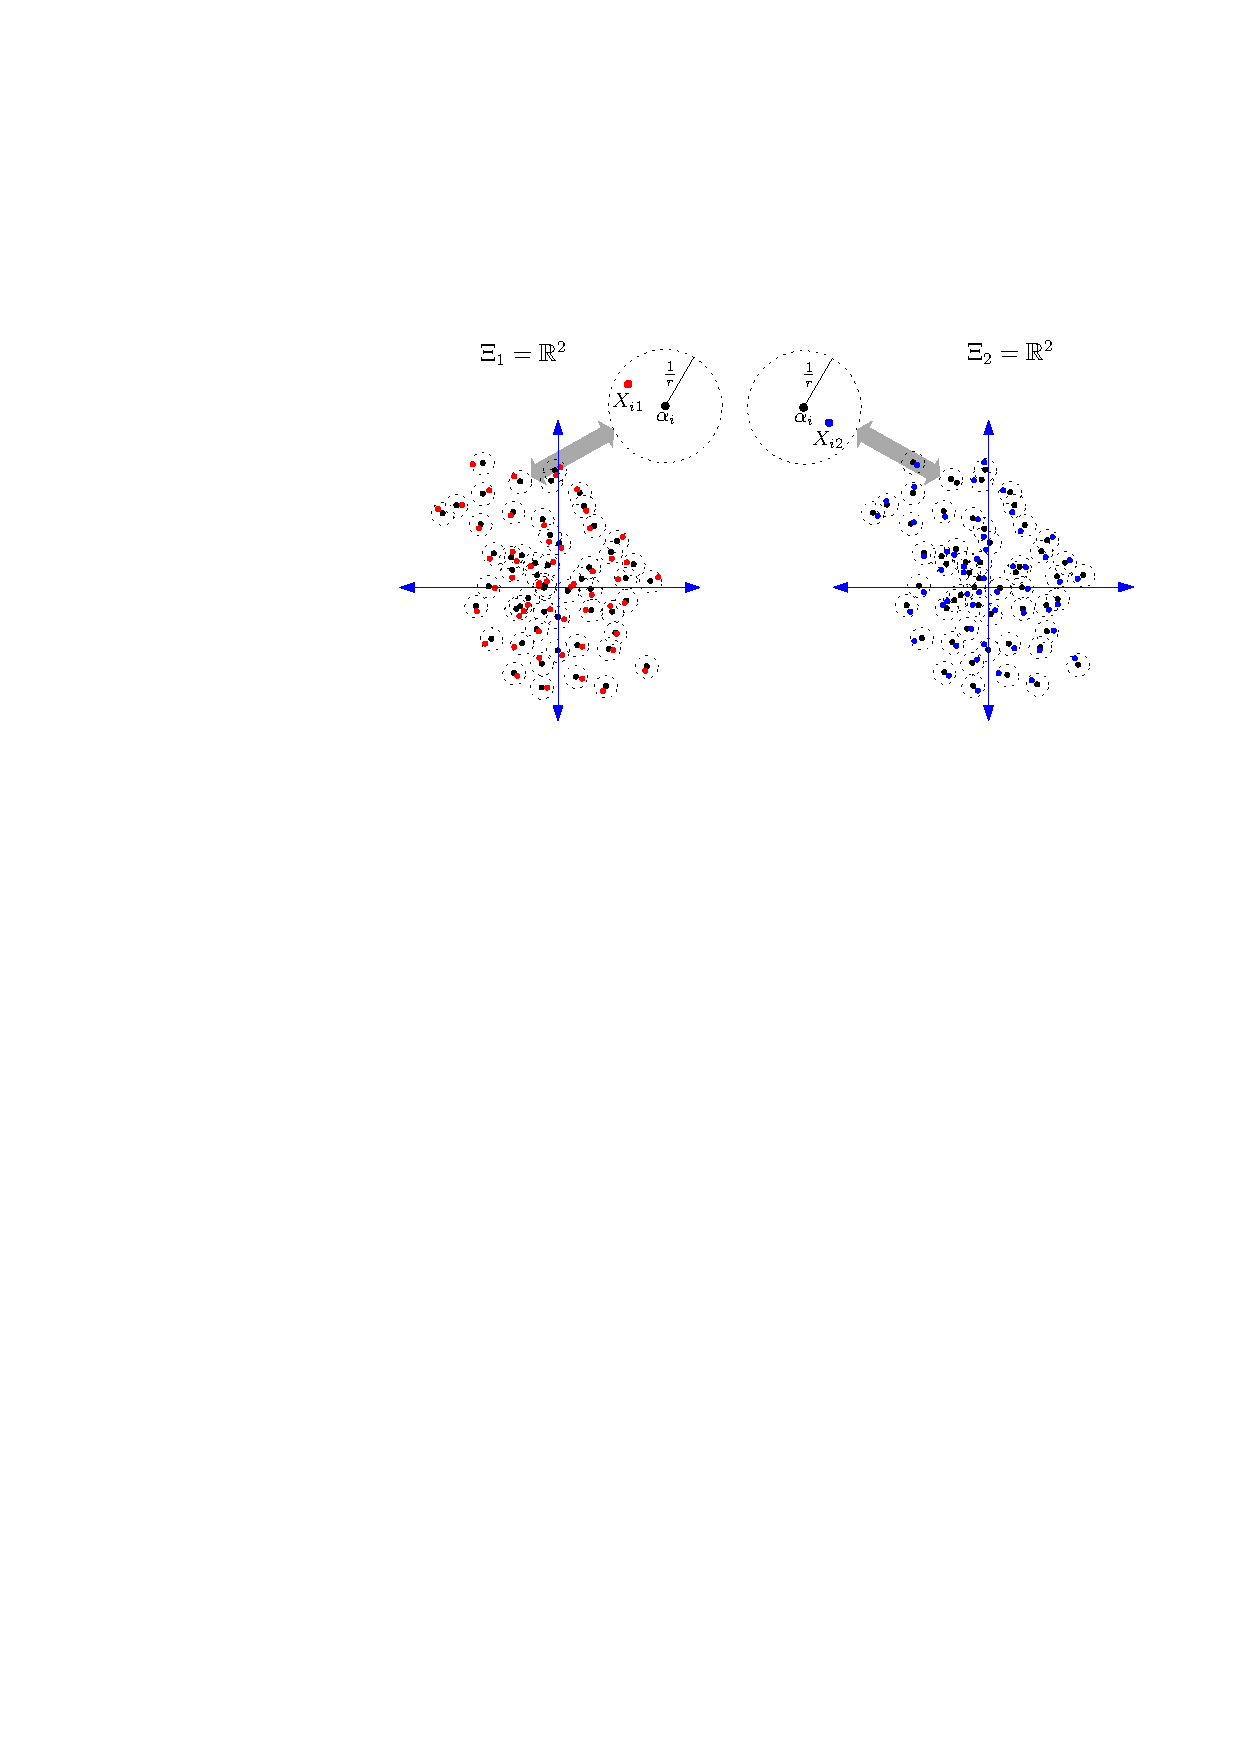
\includegraphics[scale=0.75]{MVN_alpha_r_multiple_sancar.pdf}
    \caption{For the  Gaussian setting (Section \ref{subsec:GaussianSet}), the $\alpha_i$ are denoted by black points and the $X_{ik}$ are denoted by red and blue points respectively.}
\label{fig:Fig1}
	\end{center}
  \end{figure}

\subsection{Dirichlet setting\label{subsec:DirichletSet}}
Let $S^p=\{\bm{x}:\bm{x}\in\mathbb{R}^{(p+1)}, \sum_{l=1}^p{x_l}=1\}$ be the standard $p$-simplex in $\mathbb{R}^{p+1}$.
 Let $\Xi_1 = S^p$ and $\Xi_2 = S^p$.   Denote a vector of ones by $\bm{1}_{p+1}\in \mathbb{R}^{(p+1)}$.
  Let $\bm{\alpha}_i \sim^{iid} Dirichlet(\bm{1}_{p+1})$ represent $n$  ``objects'' and let $X_{ik} \sim^{iid} Dirichlet(r\bm{\alpha}_i+\bm{1}_{p+1})$ represent $K$ measurements. See Figure~\ref{fig:Fig2}.

 The parameter $r$ again controls the variability between ``matched" measurements.
    \begin{figure}
	\begin{center}
    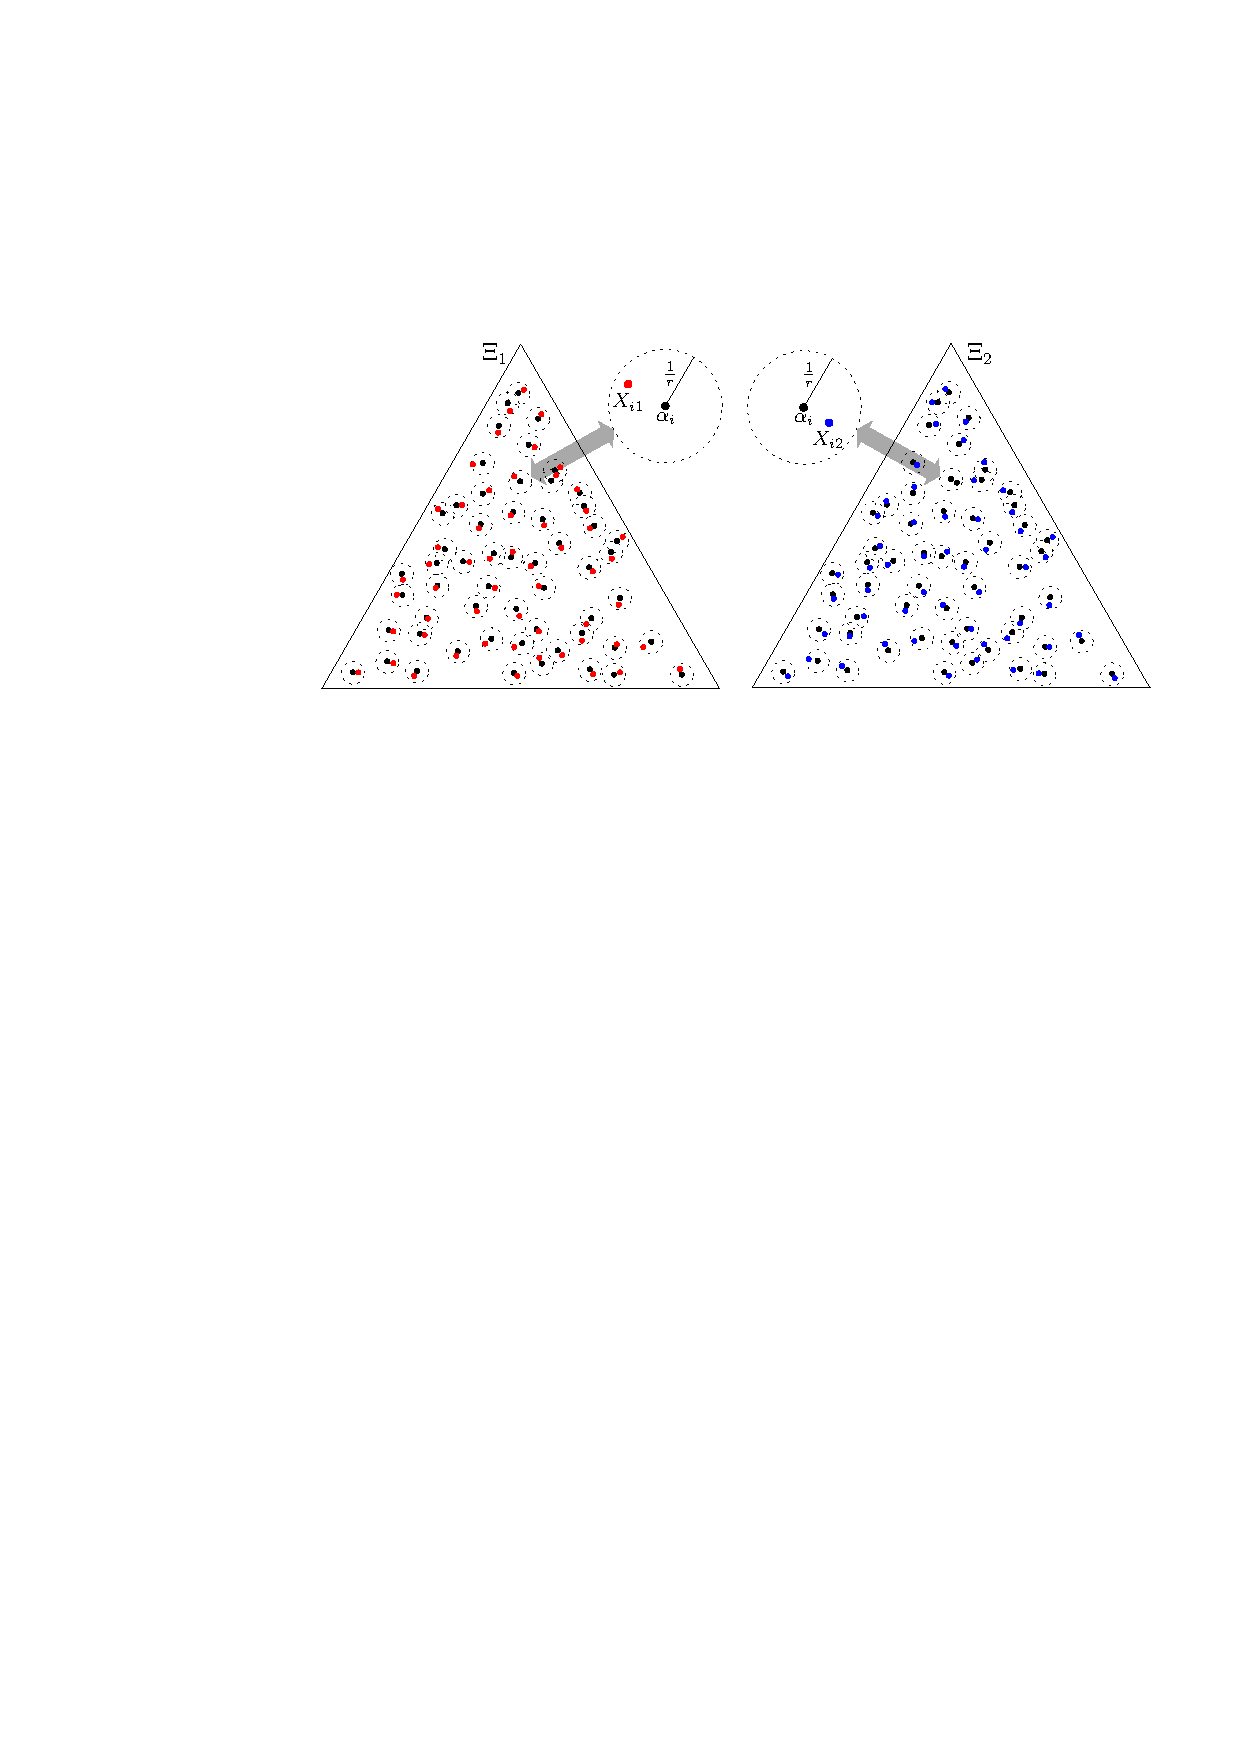
\includegraphics[scale=0.75]{Dirichlet_alpha_r_multiple_sancar.pdf}
   \caption{ For the  Dirichlet setting (Section \ref{subsec:DirichletSet}),  the $\alpha_i$ are denoted by black points and the $X_{ik}$ are denoted by red and blue points respectively.}
\label{fig:Fig2}
	\end{center}
  \end{figure}

\subsection{Noise\label{noise}}
Measurements $X_{ik}$ carry the signal that is relevant to our exploitation task. Noise dimensions can be introduced to  the measurements by concatenating a $q$-dimensional error vector whose magnitude is controlled by the parameter $c$. The noisy measurements will be  represented by the random vectors 
 \begin{equation}
\breve{X}_{ik}=[(1-c)X_{ik}\hspace{5pt} cE_{ik}]\label{eq:noise-expr}
\end{equation}
 where $E_{ik} \sim^{iid} Dirichlet(\bm{1}_{(q+1)})\label{eq:noise-model-dir} $ for the Dirichlet setting and $E_{ik} \sim^{iid} MVNormal(\bm{0} , (1+\frac{1}{r})I_{q+1}) \label{eq:noise-model-mvn} $ for the Gaussian setting. $\breve{X}_{ik}$ will be used instead of ${X}_{ik}$ for computing dissimilarities in the ``noisy" version of the problem. These noisy measurements allow the comparison of  different methods applied to the problem with respect to their robustness.
  

\section{Manifold Matching\label{sec:JOFC}}
  Our approach can be summarized as  ``manifold matching", which is defined as simultaneous ``manifold learning" and ``manifold alignment" -- identifying embeddings of multiple disparate data sources into the same low-dimensional space where joint inference can be pursued. The inference task either requires the fusion of data from disparate sources( as in the test of matchedness) or gathers performance gains from the fusion. The assumption is that the data in each measurement space lie approximately in a low dimensional manifold. An effort is made to match the low-dimensional manifolds so that matched measurements from different conditions are as close as possible to each other.  The embeddings from the dissimilarities in the measurement spaces into the commensurate space are implicit mapping from the measurement space($\Xi_k$)  to the commensurate space( $\mathcal{X}$ in ~\ref{fig:fig1}). The learning problem involves estimating these maps(whether implicit as in the dissimilarity representation of multiple sensor measurements or explicit in the  feature representation setting)  from a training data of matched measurements.


We will assume  the commensurate space  $\mathcal{X}$  is  $\mathbb{R}^d$ where $d$ is pre-specified. The selection of $d$ -- model selection -- is  a task that requires much attention and is  beyond the scope of this article.






To embed dissimilarities  $\{\Delta_k,k=1 ,\ldots,K\}$  from different conditions into a commensurate space in one step, an omnibus dissimilarity matrix  $M$ can be embedded in the low-dimensional Euclidean spaceinto one omnibus dissimilarity matrix $M$, imputing entries if necessary. Consider, for $K=2$, \begin{equation}
M=  \left[ \begin{array}{cc}
         \Delta_1 & L\\
        L^T  & \Delta_2 
     \end{array}  \right]     \label{omnibus} 
\end{equation} where $L$ is a matrix of imputed entries. One way to impute $L$ is to set it to $\frac{\Delta_1+\Delta_2}{2}$. Another choice for imputation is introduced in \ref{sec:FidComm}: the diagonal of $L$ is set to 0, the rest of the entries are $NA$ and are ignored in the optimization of MDS criterion.  
Using MDS to embed  this omnibus matrix into a  space  $\mathcal{X}$, we obtain $2n$ embedded observations $\{\tilde{y}_i^{(k)}; i=1,\ldots,n;k=1,2\}$ in a single space, with distances between the different observations consistent with the given dissimilarities. Now that the observations are commensurate, we can compute the test statistic \[
\tau=d\left(\tilde{y}_i^{(1)},\tilde{y}_j^{(2)}\right)\label{teststat}
\] for $i^{th}$ and $j^{th}$ observations under different conditions.  For ``large" values of $\tau$, we will reject the null hypothesis. We will refer to this approach as the Joint Optimization of Fidelity and Commensurability (JOFC) approach, for reasons that will be explained in Section \ref{sec:FidComm}. In this approach, the mappings   $\{ \rho_k,; k=1,\ldots,K\}$ in ~\ref{fig:fig1}  are not explicitly defined.


In any exploitation task that necessitates such an matching of manifolds or where the matching is expected to  improve performance, the omnibus embedding approach can be used  to embed the observations in a single space where they are commensurate. 


\subsection{Out-of-sample Extension}
Manifold learning algorithms computes embeddings of training data on low-dimensional manifolds, however they may not always give a map as output  to  be used to compute embeddings of new points. Applying manifold learning algorithms to the combination  of training and test data  will give us such a map, but this would need to be repeated for any new test point, and embeddings of training dissimilarities would be  partially dependent on test data. The solution is to extend the embeddings of training dissimilarities by out-of-sample embedding the test dissimilarities. 
In our hypothesis testing task, we are given dissimilarities   between a new pair of test observations and the previous $nK$ training observations. As embedding the original (in-sample) $nK \times nK$ dissimilarities between training observations doesn't result in a explicit map, we require out-of-sample embedding.  Out-of-sample extension for MDS will be used throughout this paper\cite{TrossetOOS}. 

% - given the embedded configuration $X$ of the 
%training observations and the augmented dissimilarity matrix that includes dissimilarities between test observations and %the training observations, and dissimilarities in between the training observations, oos-embedding consists of embedding
%the test points into  the existing configuration so as to be as consistent as possible with these dissimilarities (the distances %between points are as close as possible to the dissimilarities as measured by the criterion function). 
Out-of-sample embedding can be done one observation at a time, or jointly if the dissimilarities among multiple test observations are also available. 


\section{Fidelity and Commensurability constraints for Manifold Matching \label{sec:FidComm}}
Unless 
\begin{itemize}
\item the dissimilarity matrix is the Euclidean distance matrix of the original observations, and, 
\item the embedding dimension is greater or equal to the dimension of the original observations,
\end{itemize}
MDS with raw stress will not result in a perfect reconstruction  of the original observations. Note that we are not neccessarily interested in perfect reconstruction, but the best embedding for our exploitation task which is to test whether two sets of dissimilarities are ``matched". The following two criteria  are guidelines for what the manifold matching should accomplish andhelpful for optimizing the matching for the exploitation task we are to carry out.


\begin{itemize}
\item Fidelity is how well the mapping to commensurate space preserves the original dissimilarities.
Our within-condition {\em fidelity error} is given by
    \[
\epsilon_{f_{k}} = \frac{1}{{{n}\choose{2}}} \sum_{1 \leq i < j \leq n} (d(\widetilde{\bm{x}}_{ik},\widetilde{\bm{x}}_{jk})-\delta_k(\bm{x}_{ik},\bm{x}_{jk}))^2
\] 
where ${\bm{x}}_{ik}$ is the original observation of the $i^{th}$ object for the $k^{th}$  condition and $\widetilde{\bm{x}}_{ik}$ is the embedded configuration of the $i^{th}$ object  for the $k^{th}$ condition;  $d(\cdot,\cdot)$ is the Euclidean distance function (for the embedding space) and $\delta_k(\cdot,\cdot)$ is the dissimilarity function defined for objects in the $k^{th}$ condition.

\item Commensurability is how well the mapping to commensurate space preserves matchedness of matched observations. Between-condition {\em commensurability error} is given by
    \[
\epsilon_{c_{k_1k_2}} = \frac{1}{n} \sum_{1 \leq i \leq n;k_1 <k_2} (d(\widetilde{\bm{x}}_{ik_1},\widetilde{\bm{x}}_{ik_2})-{ \delta_{k_1k_2}}(\bm{x}_{ik_1},\bm{x}_{ik_2}))^2
\label{comm-error}
\]
 for conditions $k_1$ and $k_2$; $\delta_{{k_1}{k_2}}(\cdot,\cdot)$ is the (notional) dissimilarity function between measurements in  $k_1^{th}$ and $k_2^{th}$ conditions. Note that ,in general, there are $K$  within-condition fidelity error terms and $\frac{K \times (K-1)}{2}$  between-condition commensurability error terms.

Although  the between-condition dissimilarities of the same object, ${ \delta_{k_1k_2}(\bm{x}_{ik_1},\bm{x}_{ik_2}})$, are not available,  it is not unreasonable in this setting  to set ${ \delta_{k_1k_2}}(\bm{x}_{ik_1},\bm{x}_{ik_2}) = 0$ for all $i,k_1,k_2$.  So we choose diagonal  entries of $L$ in  equation \eqref{omnibus} to be all zeroes. Setting these diagonal entries to zero forces matched points to be embedded close to each other. We ignore the possibility that this choice for between-condition dissimilarities might not be optimal, in order to concentrate on the main problem.

Then, the commensurability error  term becomes
  \[
\epsilon_{c_{k_1k_2}} = \frac{1}{n} \sum_{1 \leq i \leq n;k_1< k_2} (d(\widetilde{\bm{x}}_{ik_1},\widetilde{\bm{x}}_{ik_2})))^2
\]
\end{itemize}

 There is also between-condition {\em separability error} given by
    $$\epsilon_{s_{k_1k_2}} = \frac{1}{{{n}\choose{2}}} \sum_{1 \leq i < j \leq n;k_1 <k_2} (d(\widetilde{\bm{x}}_{ik_1},\widetilde{\bm{x}}_{jk_2})-{ \delta_{k_1k_2}}(\bm{x}_{ik_1},\bm{x}_{jk_2}))^2.$$ This error will be ignored herein, due to the fact that 
$\delta_{k_1k_2}(\bm{x}_{ik_1},\bm{x}_{jk_2})$ is not  available. Although it is possible to impute these dissimilarities, the optimal  imputation is an open question and ignoring these terms provides for investigation of simpler, still open questions.


Note that the omnibus embedding approach tries to jointly optimize fidelity and commensurability , by minimization of some measure of discrepancy between the given dissimilarities (all of which are between-condition or within-condition dissimilarities) and the distances of the embedded configuration. This is most obvious in the  raw stress version of  MDS, since the individual terms can be separated according to whether they are contributing to  fidelity or  commensurability  error.

 Consider the weighted raw stress criterion $\sigma_{W}(\cdot)$ with a weighting matrix $W$, given in equation~\eqref{raw-stress}.
 The omnibus matrix $M$ we are considering is a partitioned matrix consisting of matrices from different conditions ($k={1,2}$), so we index the entries of the matrix  by 4-tuple ${i,j,k_1,k_2}$ which refers to the entry in the $i^{th}$ row and $j^{th}$ column of the submatrix in  the $k_1^{th}$  row partition and   $k_2^{th}$ column partition. For example, the entry ${M}_{2n,n}$ will have the indices $\{i,j,k_1,k_2\}=\{n,n,2,1\}$ in the new indexing scheme. $D(\cdot)$ and $W$, which are the same size as $M$, follow the same 4-tuple indexing. Then,
 
\begin{align}
\sigma_W(\cdot)  &= & &\sum_{i,j,k_1,k_2} {w_{ij{k_1}{k_2}}(d_{ij{k_1}{k_2}}(\cdot)-M_{ijk_1k_2})^2 } \notag\\
\hspace{3pt} &=& &\underbrace{\sum_{i=j,k_1<k_2}  {w_{ij{k_1}{k_2}}(d_{ij{k_1}{k_2}}(\cdot)-M_{ijk_1k_2})^2}}_{Commensurability}  \hspace{10pt}  &  + &\hspace{2.5em} \underbrace{\sum_{i<j,k_1=k_2}  {w_{ij{k_1}{k_2}}(d_{ij{k_1}{k_2}}(\cdot)-M_{ijk_1k_2})^2  }  } _{Fidelity}\notag\\
\hspace{3pt}&+&  &\underbrace{\sum_{i< j,k_1<k_2}  {w_{ij{k_1}{k_2}}(d_{ij{k_1}{k_2}}(\cdot)-M_{ijk_1k_2})^2  }  } _{Separability}\label{eq:FidCommSep}\hspace{10pt} .
\end{align}


\begin{comment}
\begin{eqnarray}{ccc}
\sigma_W(\cdot)\hspace{3pt}   &= &\sum_{i,j,k_1,k_2} {w_{ij{k_1}{k_2}}(d_{ij{k_1}{k_2}}(\cdot)-M_{ijk_1k_2})^2 } \notag\\
\hspace{3pt} &= &\underbrace{\sum_{i=j,k_1\neq k_2}  {w_{ij{k_1}{k_2}}(d_{ij{k_1}{k_2}}(\cdot)-M_{ijk_1k_2})^2}}_{Commensurability}  \hspace{10pt}  &  + & \underbrace{\sum_{i\neq j,k_1=k_2}  {w_{ij{k_1}{k_2}}(d_{ij{k_1}{k_2}}(\cdot)-M_{ijk_1k_2})^2  }  } _{Fidelity}\notag\\
\hspace{3pt}&+ &\underbrace{\sum_{i\neq j,k_1\neq k_2}  {w_{ij{k_1}{k_2}}(d_{ij{k_1}{k_2}}(\cdot)-M_{ijk_1k_2})^2  }  } _{Separability}\label{eq:FidCommSep2}\hspace{10pt} .
\end{eqnarray}
\end{comment}


Since we set ${ \delta_{k_1k_2}}(\bm{x}_{ik_1},\bm{x}_{ik_2}) = 0$, the corresponding entries of $M$ in the commensurability terms will be 0.

Since we choose to ignore  the separability error, we choose the weights for separability terms to be 0. This also means off-diagonal elements of $L$ in equation \eqref{omnibus} can be ignored. When separability terms are removed from equation \eqref{eq:FidCommSep}, the resulting equation  is a sum of fidelity and commensurability error terms:


\begin{align}
\sigma_W(\cdot)\hspace{3pt}   
\hspace{3pt}&=&\underbrace{\sum_{i=j,k_1< k_2}  {w_{ij{k_1}{k_2}}(d_{ij{k_1}{k_2}}(\cdot))^2}}_{Commensurability}  \hspace{10pt}  &  +&\underbrace{\sum_{i< j,k_1=k_2}  {w_{ij{k_1}{k_2}}(d_{ij{k_1}{k_2}}(\cdot)-M_{ijk_1k_2})^2  }  } _{Fidelity}\notag\label{eq:FidCommSep}\hspace{10pt} .
\end{align}

This motivates  referring to our omnibus embedding approach as Joint Optimization of Fidelity and Commensurabilty (JOFC).

Note that for purpose of minimization, setting all weights  ${w_{ij{k_1}{k_2}}}$ equal is equivalent to the unweighted raw stress $\sigma(X)$:
\begin{equation}
\sigma(X)=\sum_{1\leq s\leq n;1\leq t\leq n} {(d_{st}(X)-\delta_{st})^2  }\label{stress}
\end{equation}

\begin{comment}
\subsection{The incommensurability phenomenon from the viewpoint of Fidelity-Commensurability Tradeoff}

\cite{JOFC}  presented a simple example of incommensurability phenomenon, where linear projections resulted in incommensurate linear subspaces with significant probability. Due to symmetry, all projections have the the same fidelity, but there is only one pair of configurations that has  maximum commensurability. So any method that considers both fidelity and commensurability should have equal performance. This would lead one to conclude all $w$ values should be in the set of  $w^*$. 
\end{comment}

\section{Alternative Methodologies}
For the optimization of commensurability with fidelity as  secondary priority, an alternative method is Canonical Correlational Analysis (CCA)~\cite{Hardoon2004}, which aims to find linear subspaces of the Euclidean space  such that the projection of data points to those subspaces results in  vectors that are maximally correlated. CCA finds a basis for these subspaces iteratively: For each new component in the basis, CCA finds the pair of directions that maximizes correlation with the constraint that the projections along the new directions are  uncorrelated  with projections along previous components. The latter constraint results in  additional preservation of fidelity for each new direction. For the optimization of fidelity,  one can use Principal Components Analysis (PCA), which aims to find linear subspaces such that  projection of data points to those subspaces results in observation vectors that represent the original data as best as possible. To optimize commensurability as  secondary priority, one can use the projections computed by PCA to  compute a Procrustes transformation that will make the projections commensurate. Since the data is originally in a dissimilarity representation, we can directly embed in the low-dimensional space and use Procrustes Analysis to find a mapping between the two separate embeddings. The equivalence of PCA and Classical Multidimensional Scaling~\cite{CMDS} under certain conditions suggests that this approach is the right analog of Procrustes $\circ$ PCA to utilize when in a dissimilarity setting. 

 The omnibus embedding  approach is expected to be more powerful for the exploitation task than either of  the sequential optimizations, since the exploitation task (testing matchedness) requires both optimization of fidelity and commensurability.

\subsection{Procrustes Analysis on Multidimensional Scaling Embeddings\label{subsec:PoM}} 
Since separate  condition dissimilarities are available, a straightforward approach is to embed each conditional dissimilarity matrix, $\Delta_1$ and $\Delta_2$, separately  in  $d$-dimensional Euclidean space (call these embedded configurations $X_1$ and $X_2$, respectively) and then find a mapping function $\rho :\mathbb{R}^{d}\rightarrow\mathbb{R}^{d}$ that maps each point in $X_2$ to approximately its corresponding point in $X_1$. This approach can be seen as a specific example of the general setting where the commensurate space is d-dimensional  Euclidean space and $\rho_1$ in  ~\ref{fig:fig1} is the identity map. 

Estimation of $\rho$ is carried out using  Procrustes Analysis  on training data. Procrustes Analysis~\cite{Sibson} finds a orthonormal matrix $\mathbf{Q}^*$ that minimizes the sum of squared distances between the  target configuration $X_1$ and  the configuration $X_2$ transformed by $\mathbf{Q}^*$, i.e.,
 \[\mathbf{Q}^* = \argmin_{Q^TQ = I} \|X_1 - X_2Q\|_F\] 
 where $\|\cdot\|_F$ is the Frobenius norm on matrices. The map $\rho$ estimated by the linear map $\mathbf{Q}^*$   makes the separate MDS embeddings as commensurate as possible. Once such a mapping is computed, one can out-of-sample embed  new dissimilarities for each condition (separately)  and  use $\mathbf{Q}^*$ to make the embeddings commensurate.
One can then compute the test statistic $\tau$ (the distance between commensurate embeddings) for  the hypothesis testing problem. We will refer to this approach as P$\circ$M - Procrustes $\circ$MDS.

Note that the Procrustes transformation $\mathbf{Q}^*$  is limited to  a linear transformation consisting of rotation and reflection and possibly also scaling components. The optimal mapping might  very well be   non-linear. If we allow  a larger class of mappings to be considered, we would have a smaller model bias for the mapping function, but we would be paying for it  in the form of larger variability. By only considering the class of linear transformations, we are able  to learn $\mathbf{Q}^{*}$ with our limited dataset.


\subsection{Canonical Correlational  Analysis on Multidimensional Scaling Embeddings} 

Again MDS is used  to compute embedding configurations, $ X_1$ and $X_2$. We want to embed into the highest dimensional space  possible ($\mathbb{R}^{d'}$ where $d'=p+q$ for our Gaussian and Dirichlet settings)  to  preserve as many of the signal dimensions as possible (at the risk of possibly including  some noise dimensions). CCA~\cite{Hardoon2004}, then,  yields two mappings $\mathcal{U}_1$ and $\mathcal{U}_2$ that map these embeddings in $\mathbb{R}^{d'}$ to  the low-dimensional commensurate space ($\mathbb{R}^d$). 

\subsubsection*{Canonical Correlational Analysis}

 Let $X$ and $Y$ be two $s$-dimensional random vectors. If  one wants to find  the pair of linear projection operators $U_1:\mathbb{R}^s \rightarrow  \mathbb{R}$, $U_2 :\mathbb{R}^s \rightarrow  \mathbb{R}$ that maximize correlation between the projections of   $X$ and $Y$, CCA finds the solution as stated in the  optimization problem
$$
{\hat{u}_1 ,\hat{u}_2}=\arg\max_{u_1\in\mathbb{R}^s,u_2\in\mathbb{R}^s} {\frac{E[u_1^{T}XY^Tu_2]}{{E[u_1^{T}XX^T u_1]}{E[u_2^{T}YY^T u_2]}}}$$
with the constraints $E[{u_1^{T}XX^T u_1}]=1 , E[{u_2^{T}YY^T u_2}]=1$ for uniqueness. The constraints simplify the optimization function to $$
\arg\max_{u_1\in \mathbb{R}^s,u_2\in \mathbb{R}^s} {E[u_1^{T}XY^Tu_2]}.$$

If the projections are to a pair of $d$-dimensional linear subspaces, the additional pairs of projection vectors can be computed sequentially, with the constraints that the projections along the new directions are uncorrelated with  projections along previous directions. That is, $i^{th}$ pair of directions  that maximize correlation is computed by 
$$
{\hat{u}_{1(i)},\hat{u}_{2(i)}}=\arg\max_{u_{1(i)},u_{2(i)}\in\mathbb{R}^s} {E[u_{1(i)}^{T}XY^Tu_{2(i)}]}.$$ subject to constraints $E[{u_{1(i)}^{T}XX^T u_{1(i)}}]=1$ , $E[{u_{2(i)}^{T}YY^T u_{2(i)}}]=1$, $E[{u_{1(i)}^{T}XX^T u_{1(j)}}]=0$,  
   $ E[{u_{2(i)}^{T}YY^T u_{2(j)}}]=\nolinebreak0$ $\forall \quad  j=1,\ldots,i-1$. For sample CCA, $E[XX^T]$,$E[YY^T]$ and $E[XY^T]$ are replaced with their sample estimates. The direction vectors ${\hat{u}_{1(i)},\hat{u}_{2(i)}}, i=1,\ldots,d $ form the rows of projection matrices which represent the mappings $\mathcal{U}_1$ and $\mathcal{U}_2$. 


Note that $s$, the dimension of $X$ and $Y$, is the embedding dimension $d'$  in the CCA approach. 


As in P$ \circ $M, new dissimilarities are out-of-sample embedded and mapped to a commensurate  space by maps provided by CCA. We can now compute the test statistic  and reject the null hypothesis for ``large'' values of the test statistic $\tau$  as in Section \ref{subsec:PoM}.


\subsection{Relation of $P\circ M$ and Joint Optimization of Fidelity and Commensurability} 

Suppose we let $w_{ijk_1k_2}=w$ for commensurability terms and $w_{ijk_1k_2}=1-w$ for fidelity terms in equation \eqref{eq:FidCommSep}. For the resulting weight matrix $W$, define 
\begin{equation}
f_w(D(\cdot),M) = \sigma_W(\cdot) \label{fid-comm-tradeoff-func}
\end{equation}
 where $M$ is the omnibus matrix obtained from  a given pair of dissimilarity matrices, $\Delta_1$ and $\Delta_2$, as in equation \eqref{omnibus}.   As $w$ goes to 0, the configuration embedded by JOFC converges to a configuration equivalent to (up to rotation and reflection)  the configuration embedded by P$\circ$M.


\begin{thm}
Define $\sigma(\cdot)=\sigma_{W=\bm{1}}(\cdot)$ (unweighted raw stress) where $\bm{1}$ is a matrix of 1's.
 Let $\mathbf{X}_1$ and $\mathbf{X}_2$ be the corresponding $n\times p$ configuration matrices with column means of $\bm{0}$ (obtained from separately embedding  $\Delta_1$ and $\Delta_2$ by minimizing the raw stress $\sigma(\cdot)$ ). 
Let  $\mathbf{Q}=\argmin_{\mathbf{P^T}\mathbf{P}=\mathbf{P}\mathbf{P^T}=\mathbf{I}}||{\mathbf{X}_1-\mathbf{X}_2}\mathbf{P}||^2$ ,   $\mathbf{\tilde{X}}_2= \mathbf{X}_2\mathbf{Q}$, 
and let  
$\mathbf{X}=\left[\begin{array}{c}
\mathbf{X}_1\\
\mathbf{\tilde{X}}_2
\end{array}\right]$.

For $w>0$, let $\mathbf{Y}_{w} = \left[\begin{array}{c}
\mathbf{Y}_1\\
\mathbf{Y}_2
\end{array}\right]$  be  a $2n \times p$ configuration matrix obtained by minimization of 
$ f(\mcY, M) =(1-w)\left({\sigma{(\mcY_1)}}+{\sigma{(\mcY_2)}}\right)+w||{\mcY_1-\mcY_2}||^2 $ with respect to  $\mcY=\left[\begin{array}{c}
\mcY_1\\
\mcY_2
\end{array}\right]$ with the constraint that $\mcY_1$ and $\mcY_2$ are two $n \times p$ configuration matrices having column means of $\bm{0}$. Then, $$lim_{w\rightarrow0}\mathbf{Y}_{w}=\mathbf{X}\mathbf{R}$$ for a $p\times p$ orthonormal matrix $\mathbf{R}$. ($\mathbf{R}$ is a transformation matrix with a rotation and possibly a reflection component.)
\end{thm}
 

\subsection{Relation of CCA and Commensurability} 

\begin{thm}
Let $ \mathcal{U}$ be the set of all orthogonal d-frames 
(ordered set of d linearly independent vectors) of $R^{d'}$. 
Let $X_1$ and $X_2$  be two $n\times d'$ (configuration) matrices that are perfectly ``matched"
 (there exists a transformation matrix $\mathbf{Q}$ such that $\|   X_1\mathbf{Q}  -X_2 \|=0$).
If commensurability is  defined as
in equation~\eqref{comm-error},
 where  the embedded configurations are $\tilde{X_1}=X_1U_1$ and $\tilde{X_2}=X_2U_2$ for some  $U_1\in \mathcal{U}$ and $U_2\in  \mathcal{U}$,
and   the original dissimilarities are $D(X_1)$ and $D(X_2) $,
 CCA on $X_1$ and $X_2$ gives $\mathbf{U}_1\in\mathcal{U}$ and  $\mathbf{U}_2\in\mathcal{U}$, 
 the two elements of $\mathcal{U}$ that maximize commensurability, subject to $U_1^{T}X_1^{T}X_1U_1=I_d$ and $U_2^{T}X_2^{T}X_2U_2=I_d$ ($I_d$ is the $d \times d$ identity matrix).
\end{thm}



\section{Related Work \label{sec:RelatedWork}}
There have many efforts toward solving ``manifold alignment", which is a related  problem. ``Manifold alignment" seeks to find correspondences between observations from different ``conditions". The setting that is most similar to ours is the semi-supervised setting, where a set of correspondences are given and the task is to find correspondences between a new set of points in each condition. In contrast, our hypothesis testing task is to determine whether any given pair of points is ``matched" or not. The proposed solutions follow a common approach in that they look for a common commensurate or a latent space, such that the representations (possibly projections or embeddings) of the observations in the commensurate space match.

Wang and Mahedavan~\cite{Wang2008} suggest an  approach that uses embedding followed by Procrustes Analysis to find a map to a commensurate space. Given a paired set of points, Procrustes Analysis~\cite{Sibson}, finds a transformation from one set of points to another in the same space that minimizes sum of squared distances, subject to some constraints on the transformation. In the case mentioned in \cite{Wang2008}, the paired set of points are corresponding low-dimensional embeddings of kernel matrices.   For the embedding step, they made the choice of using Laplacian Eigenmaps, though their algorithm allows for any appropriate embedding method.

 Zhai et al.~\cite{Zhai2010}  finds two projection matrices to minimize three terms in an energy function similar to our JOFC approach (see Section \ref{sec:JOFC}). One of the terms is the \emph{correspondence preserving term} which is the sum of the squared distances between corresponding points and is analogous to our commensurability error term. The other two terms are \emph{manifold regularization terms} and consist of the reconstruction error for a Locally Linear Embedding of the projected points. These terms, analogous to fidelity, make sure the projections in the lower dimension retain the structure of the original points. For fidelity error terms in our setting, this is done by preserving dissimilarities. For manifold regularization terms, this is done by preserving the local neighborhood of points, such that close points are not mapped apart.
Ham and Lee solve the problem in semi-supervised setting by a similar approach, by minimizing a cost function of three terms, two terms for fidelity of embedding, one term of commensurability.


Another view to look at the data from different sources is to consider disparate data as different views to be reconciled. According to this view, for observations of $n$ objects under $K$ conditions, $n$ points are embedded instead of $nK$ points. Choi et al.\ \cite{Choi:2008:MIM:1619995.1620064} use the Markov random walk interpretation of multiple kernel matrices to combine into one kernel matrix.  Many other ``Multiple Kernel Learning"  methods exist in the literature~\cite{McFee:2011:LMS:1953048.1953063,Lin2009,Lanckriet2004}.

Another approach is Three-way Multidimensional scaling\cite{3wayNMDS,borg+groenen:1997}.
 This approach assumes the  different ``conditions" of the data are linear transformations of a single configuration and aims to find this single configuration. For our setting, one would first embed the in-sample dissimilarities via the three-way MDS, which would give as the linear transformations that map from group configuration to individual configurations under each condition. This is followed by out-of-embedding the OOS dissimilarities, and use the inverse of the transformation matrices to find the out-of-sample embeddings with respect to the group configuration. Since the out-of-sample embeddings are commensurate, the test statistic can be computed as the distance between the OOS embeddings. 

%According to our ideas of tradeoff between fidelity and commensurability, this always maximizes commensurability without regard for fidelity and the constraint of the linear transformations between the group and condition configurations allows the approach to recoup some fidelity. 


\section{Fidelity and Commensurability Tradeoff}
The major question  addressed in this work is whether in the tradeoff between preservation of fidelity and preservation of  commensurability , there is an optimal point for our hypothesis testing task.  The weights in raw stress allow us to answer this question relatively easily. Since in equation \eqref{eq:FidCommSep},  each term indexed with $i$, $j$ is either a fidelity or a commensurability term, setting $w_{ij}$ to $w$ and $1-w$  for commensurability  and fidelity  terms respectively will allow us to control the importance of fidelity and commensurability terms in the optimization by varying $w$. 
\begin{align*}
\sigma_W(X)&=  f_w(D(X),M) & &\\
&=  \underbrace{\sum_{i=j,k_1\neq k_2}  {w(d_{ij{k_1}{k_2}}(X))^2}}_{Commensurability} & +\hspace{2em} & \underbrace{\sum_{i<j,k_1=k_2}  {(1-w)(d_{ij{k_1}{k_2}}(X)-M_{ijk_1k_2})^2  }  } _{Fidelity}\\
&=  \left(w\right)\left(n\right) \epsilon_{c_{k_1=1,k_2=2}} & +\hspace{2em} & (1-w){{n}\choose{2}} ( \epsilon_{f_{k=1}}+\epsilon_{f_{k=2}} )
\end{align*}

Our expectation is that there is a $w^*$ that is optimal for the specific exploitation task (has the best power in hypothesis testing). In fact, our exploratory simulations confirm the power of the tests varies with varying $w$ and indicate the range where the optimal  $w^*$ lies.



\section{Definition of  $w^*$}

Let $\mathbf{F}_m$ be the joint distribution of
$X_m= \left[
 \begin{array}{c}
X_{1m}\\
X_{2m}
\end{array}
\right]$ and 
$\mathbf{F}_u$ be the  joint distribution of
$X_u= \left[
 \begin{array}{c}
 X_{1u}\\
 X_{2u} 
\end{array}
\right]$
 where   $X_{1m},X_{2m}$ are the random vectors of dimension $d'$ for the matched observation pair and $X_{1u},X_{2u}$ are the random vectors of dimension $d'$ for the unmatched data pair.   The constraint on  $\mathbf{F}_m$ is that  correlation  matrix of $X_{1m},X_{2m}$ is non-zero, while  the constraint on $\mathbf{F}_u$   is that correlation  matrix of $X_{1u},X_{2u}$ is zero.

Let $\mathcal{T}$ denote  the random variable for a data matrix ($2n\times d'$) for an  i.i.d. sample of  
$\left[ \begin{array}{c}
X_{1m}\\
X_{2m}
\end{array}
\right]$ and let  $\mathbf{T}_{mc}$  denote realization of $\mathcal{T}$ for any Monte Carlo replicate.


For the exploitation task at hand, it is assumed that either
\begin{itemize}
\item  we are given a sample of $\mathcal{T}$ ($\mathbf{T}_{mc}$) and a sample of $X_m$ and  $X_u$ 
$\left(\bm{x_m}=\left[
 \begin{array}{c}
\bm{x}_{1m}\\
\bm{x}_{2m}
\end{array}
\right] ,\bm{x_u}=\left[
 \begin{array}{c}
 \bm{x}_{1u}\\
 \bm{x}_{2u} 
\end{array}
\right]\right)$ 
 and  we compute Euclidean distances between  $\bm{x}_{.m}$ and the rows in  $\mathbf{T}_{mc}$  and Euclidean distances between  $\bm{x}_{.u}$ and the rows in  $\mathbf{T}_{mc}$ to form  dissimilarity matrices $\Delta_m$ and $\Delta_u$, or
\item we are given values of  dissimilarity matrix-valued function $D$ of  the sample of $X_m$, $X_u$ and $\mathbf{T}_{mc}$: $$
\mathbf{\Delta_m} = D \left( \left[
 \begin{array}{c}
\mathbf{T}_{mc}  \\
\bm{x}_{1m}\\
\bm{x}_{2m}\\
\end{array}
\right]
\right)
$$
$$
\mathbf{\Delta_u}=D \left( \left[
 \begin{array}{c}
\mathbf{T}_{mc}  \\
\bm{x}_{1u}\\
\bm{x}_{2u}\\
\end{array}
\right]
\right)
$$
where the  $(s,t)^{th}$ entry of $D(\cdot)$   ($d_{st}(\cdot)$ in equation \eqref{raw-stress})  is the Euclidean distance between the $s^{th}$ and $t^{th}$ rows of its argument.
\end{itemize}

Either way, we define the disssimilarity matrices $\Delta_{m} \left(\left[
\begin{array}{c}
\mathcal{T} \\
X_{1m} \\
X_{2m} 
\end {array}
\right]
\right)$  and 
 $\Delta_{u} \left(\left[
\begin{array}{c}
\mathcal{T}\\
X_{1u} \\
X_{2u}
\end {array}
\right]\right)$ as two matrix-valued random variables $\Delta_{m}:\Omega \rightarrow \mathbf{M}_{n\times n} $,$\Delta_{u}:\Omega \rightarrow \mathbf{M}_{n\times n} $  for the probability space $(\Omega,\mathcal{B},\mu)$.

 The criterion function for the embedding is $\sigma_W(\cdot) =f_w(D({\cdot}),\Delta)$. The embedding for the unmatched pair ${\hat{X}_{1u},\hat{X}_{2u}}$  is 
 \[
{\hat{X}_{1u},\hat{X}_{2u}}
=\argmin_{\acute{X}_{1u}, \acute{X}_{2u}}\left[\min_{\mathbf{\acute{T}}}
{f_w\left(
D\left(
\left[
\begin{array}{c}
\acute{\mathbf{T}} \\
\acute{X}_{1u} \\
\acute{X}_{2u}
\end {array}
\right]
\right),
\Delta_{u}
\right)
}
\right]
\]
where there is an implicit dependence on $\mathbf{T}$, because $\Delta_{u}$ depends on $\mathbf{T}$. 
A similar expression gives the embedding for the matched pair  
${\hat{X}_{1m},\hspace{0.5em}\hat{X}_{2m}}=\argmin_{\acute{X}_{1m}, \acute{X}_{2m}}\left[\min_{\mathbf{\acute{T}}}
{f_w\left(
D\left(
\left[
\begin{array}{c}
\acute{\mathbf{T}} \\
\acute{X}_{1m} \\
\acute{X}_{2m}
\end {array}
\right]
\right),
\Delta_{u}
\right)
}
\right]$.
 Assuming these minima exist and are unique, the mappings $\hat{X}_{1m}:\omega\rightarrow \mathbf{R}^{d'}$,  $\hat{X}_{2m}:\omega\rightarrow \mathbf{R}^{d'}$ , $\hat{X}_{1u}:\omega\rightarrow \mathbf{R}^{d'}$, 
$\hat{X}_{2u}:\omega\rightarrow \mathbf{R}^{d'}$ are  measurable maps,  $\hat{X}_{1m}$ , $\hat{X}_{2m}$ , $\hat{X}_{1u}$, $\hat{X}_{2u}$ are random vectors. 
Define $F_Y$ as the   cumulative distribution function of  $Y$ where $Y$ can be  any function of $\hat{X}_m$ or $\hat{X}_u$.




 Then $$\beta_{\alpha}\left( w\right)=1-F_{d(\hat{X}_{1u},\hat{X}_{2u})}(F_{d(\hat{X}_{1m},\hat{X}_{2m})}^{-1}(1-\alpha)).$$

 Finally, define $$w^{*}=argmax_w{\beta_{\alpha}\left( w\right)}. $$


Even for  given $\mathbf{F}_u,\mathbf{F}_m$,   $w^*$ must be defined with respect to the value of allowable type I error rate $\alpha$.  For two different $\alpha$ values, it is quite possible that $\beta_{\alpha_1}(w_1)>\beta_{\alpha_1}(w_2)$  and $\beta_{\alpha_2}(w_1)<\beta_{\alpha_2}(w_2)$. This can be observed in results in Section \ref{sec:Simulation Results}.  
Investigation of some  properties of $w^{*}$  is included in section  \ref{sec:Simulation Results} .
We have defined $w^*$ to be the argmin of  the power function with respect to $w$ and some important questions about $w^*$ are  related to the nature of this function $\beta_{\alpha}\left( w\right)$.

Note that in a general setting, finding the exact value of $w^*$ is intractable. The estimate $\hat{w}^*$ will be based on noisy evaluations of $\beta(w^*)$.  A Monte Carlo simulation is run in   \ref{sec:Simulation Results} 
to find the estimate of this function at various values of $w$.

\begin{comment}
A closed-form expression for this function will be hard to find  even in the most simple of cases. So consider the estimate from the Monte Carlo simulation $\beta^{(m)}_{\alpha}(w)$ for the estimate computed from $2m$ testing pairs, m matched pairs and m unmatched pairs. We will consider an arbitrary element $\omega$ of sample space $\Omega$. By law of large numbers, $\beta^{(m)}_{\alpha}\rightarrow\beta_{\alpha}(w)$ pointwise.  We will omit $w$ from the expressions of the functions. Suppose the test statistic values  are $T_0^{i}$, $T_A^{i}$ $i=1,\ldots,m$  respectively for matched and unmatched test pairs. Note that $\beta^{(m)}_{\alpha}$ can be written as $\sum_{j=1}^m I(T_A^{j}>T_0^{(i)})$ where $T_0^{(i)}$ is the $i=\lceil {m*(1-\alpha)} \rceil^{th}$ order statistic of $T_0^{i},i=1,\ldots,m$. Replacing the indicator function with the unit step function
\[
\beta^{(m)}_{\alpha}=\sum_{j=1}^m u(T_A^{j}-T_0^{(i)})
\]

Instead of this function which is not differentiable with respect to  $T_0^{i}$ and  $T_A^{i}$, consider the ``soft" approximation of this function with the sigmoid function
\[
\mathcal{B}_{alpha}^{(m)}=\sum_{j=1}^m \sigma(T_A^{j}-T_0^{(i)})
\]

Now we can consider the derivative  $\frac{d\mathcal{B}_{\alpha}^{(m)}}{dw}$, which is equal to 
\[
\frac{d\mathcal{B}_{\alpha}^{(m)}}{dw}=\sum_{j=1}^m \frac{\partial \sigma(T_A^{j}-T_0^{(i)})}{\partial T_A^{j}} \frac{\partial T_A^{j}}{w}+ \sum_{j=1}^m \frac{\partial \sigma(T_A^{j}-T_0^{(i)})}{\partial T_0^{j}} \frac{\partial T_0^{j}}{\partial w}
\] if the partial derivatives exist.
To prove differentiability of $\beta_{\alpha}\left( w\right)$ , we refer to Theorem 5.3.3 in \cite{ElClassAnalysis-5-3-3}, which requires the pointwise convergence of   $\mathcal{B}_{alpha}^{(m)}$   to  $\beta_{\alpha}\left( w\right)$ , that $\frac{d\mathcal{B}_{alpha}^{(m)}}{dw}$ are continuous and that they  converge \emph{uniformly} to a function $g$. Since the sigmoid function $\sigma(\cdot)$ is continously differentiable, we can focus on our attention  on $ \frac{\partial{T_0^{j}}}{\partial{w}}$ and $ \frac{\partial{T_0^{j}}}{\partial{w}}$. We show  that while the embedded configurations of points might not be  continuous everywhere (we present a particular example in \ref{subsubsec:Discontinuity}) $T_0^{j}$ and $T_A^{i}$ is nevertheless continuous with respect to $w$. 
\end{comment}


 
\subsection{Continuity of $\beta(\cdot)$} 
 Consider $\beta_{\alpha}(\cdot)$ as a function of $w$. We can write it as $P\left[T_a(\cdot)>c_{\alpha}(\cdot)\right]$ where $c_{\alpha}(\cdot)$ is the critical value for level $\alpha$. Instead of proving the continuity of $\beta_{\alpha}(\cdot)$
 %stochastic process whose sample path is  a function of $w$ where the randomness comes from $\Delta_{m}$, $\Delta_{u}$ and %$\mathcal{T}$ . 
 we will make use of the area under the curve measure as a surrogate: $$AUC(w)=P\left[T_a(w)>T_0(w)\right]$$ where $T_a(\cdot)$ and $T_0(\cdot)$ can also be regarded as  stochastic processes whose sample paths are continuous functions of $w$ except at a finite number of points in $(0,1)$. By  assuming stochastic continuity of $T_a(w)$ and $T_0(w)$ in the interval $(0,1)$, ie assuming the probability of a jump discontinuity of $T_0(w)$ at a particular $w_0$ is 0, we will prove the continuity of $AUC(w)$.


\begin{thm}
Let $T(\cdot)$ be  a stochastic process indexed by $w$ in the interval (0,1). Assume  the process is continuous in probability  (stochastic continuity)   everywhere in the interval  i.e.
$$ \forall a>0 \quad  \lim_{\delta \rightarrow 0} Pr\left[\|T(w+\delta)-T(w) \|>a \right] \rightarrow 0 \quad(*)$$ 

 $\forall w\in (0,1)$.

Then,

for any $w>0, \epsilon>0$, there exist $\delta_{\epsilon}$ $$\| Pr\left[T(w+\delta_{\epsilon})>0 \right]- Pr\left[T(w)>0 \right]\|<\epsilon .  $$

and 

$Pr \left[ T(w)>0\right]$ is continuous with respect to $w$.
\end{thm}

\begin{proof}
We know there exists a $\delta$ for any given $\epsilon>0$ satisfying (*). For any such $\delta$, consider the difference of the probabilities of the two events  $T(w)>0$ and $T(w+\delta)>0$ for any $w$.
\begin{eqnarray*}
\| Pr\left[T(w+\delta)>0 \right]- Pr\left[T(w)>0 \right]\| & = & \| Pr\left[T(w+\delta)>0   \cap T(w) \leq 0 \right] + Pr\left[T(w+\delta)>0   \cap T(w) > 0 \right] - \\
& & (Pr\left[T(w+\delta)> 0   \cap T(w) > 0 \right]+ Pr\left[T(w+\delta)\leq 0  \cap T(w) > 0\right]\| \\
& = & \| Pr\left[T(w+\delta)>0   \cap T(w) \leq 0 \right]- Pr\left[T(w+\delta)\leq 0  \cap T(w) > 0\right]\| \\
&= &\| Pr\left[T(w+\delta) - T(w)  > 0 \right]-  Pr\left[ T(w)- T(w+\delta)  > 0   \right]\|\\
& \leq & \| Pr\left[\{T(w+\delta) - T(w)  > 0\} \vee \{T(w)- T(w+\delta)  > 0 \}  \right]\|\\
& = & Pr\left[\|T(w+\delta) - T(w)\| >0 \right] \\
& < & \epsilon
\end{eqnarray*} 
.
\end{proof}

\begin{cor}{
 $AUC(w)=P\left[T_a(w)-T_0(w) >0 \right]$ is continuous with respect to $w$.}
\end{cor}
\begin{proof}
 $Pr\left[T(w)>0 \right]$  as a function of $w$ is continuous with respect to $w$.  Let $T(w)=T_a(w)-T_0(w)$.
\end{proof}


 The main assumption we used is the stochastic continuity of $T_0(w)$ and $T_a(w)$ . This is equivalent to  a jump discontinuity at $w$ under the probability distribution that governs the data has measure  zero. Under a continuous distribuition  In the constructed example in \ref{subsubsec:Discontinuity}, we assume a certain symmetry in the realized configuration, which gave us a discontinuity in the embedding configuration (and therefore the test statistic) at a particular point of $w$.  Any change in this symmetry should give a discontinuity at a different $w$.


\begin{comment}
For the theorem to hold, a uniform bound on the derivatives with respect to $w$.
One of the important questions to be explored is   the uniqueness of  $w^*$.   The first step in answering this question is to determine whether $\beta(w)$ is multimodal. In the two settings we described,   $\beta(w)$ seems to have one maxima that is $\in (0,1)$.
\end{comment}

\begin{comment}
First, note that  $\beta(w)$ is continuous with respect to $w$ and locally convex  with respect to embedding coordinates $\hat{X}_{.}$
\end{comment}

\subsubsection{ A short detour : Discontinuity in weighted raw stress OOS configurations\label{subsubsec:Discontinuity}}

Note that it is possible to have multiple local minima in the embedding step(see example in \cite{TrossetLocalMin}). We will construct an example  where $w$ controls which of the local minima is the global minimum among the configurations of $\hat{X}_{.}$. 


Consider five in-sample points in $\mathbb{R}^2$ with locations $X_1=(0,0)$, $X_2=(1,0)$, $X_3=(1,1)$
 and $X_4=(1,0)$, $X_5=(.5,.5)$ and two out-of-sample  points with coordinates $X_6=(1,0)$ and $X_7=(0,1)$.
 \begin{figure}
 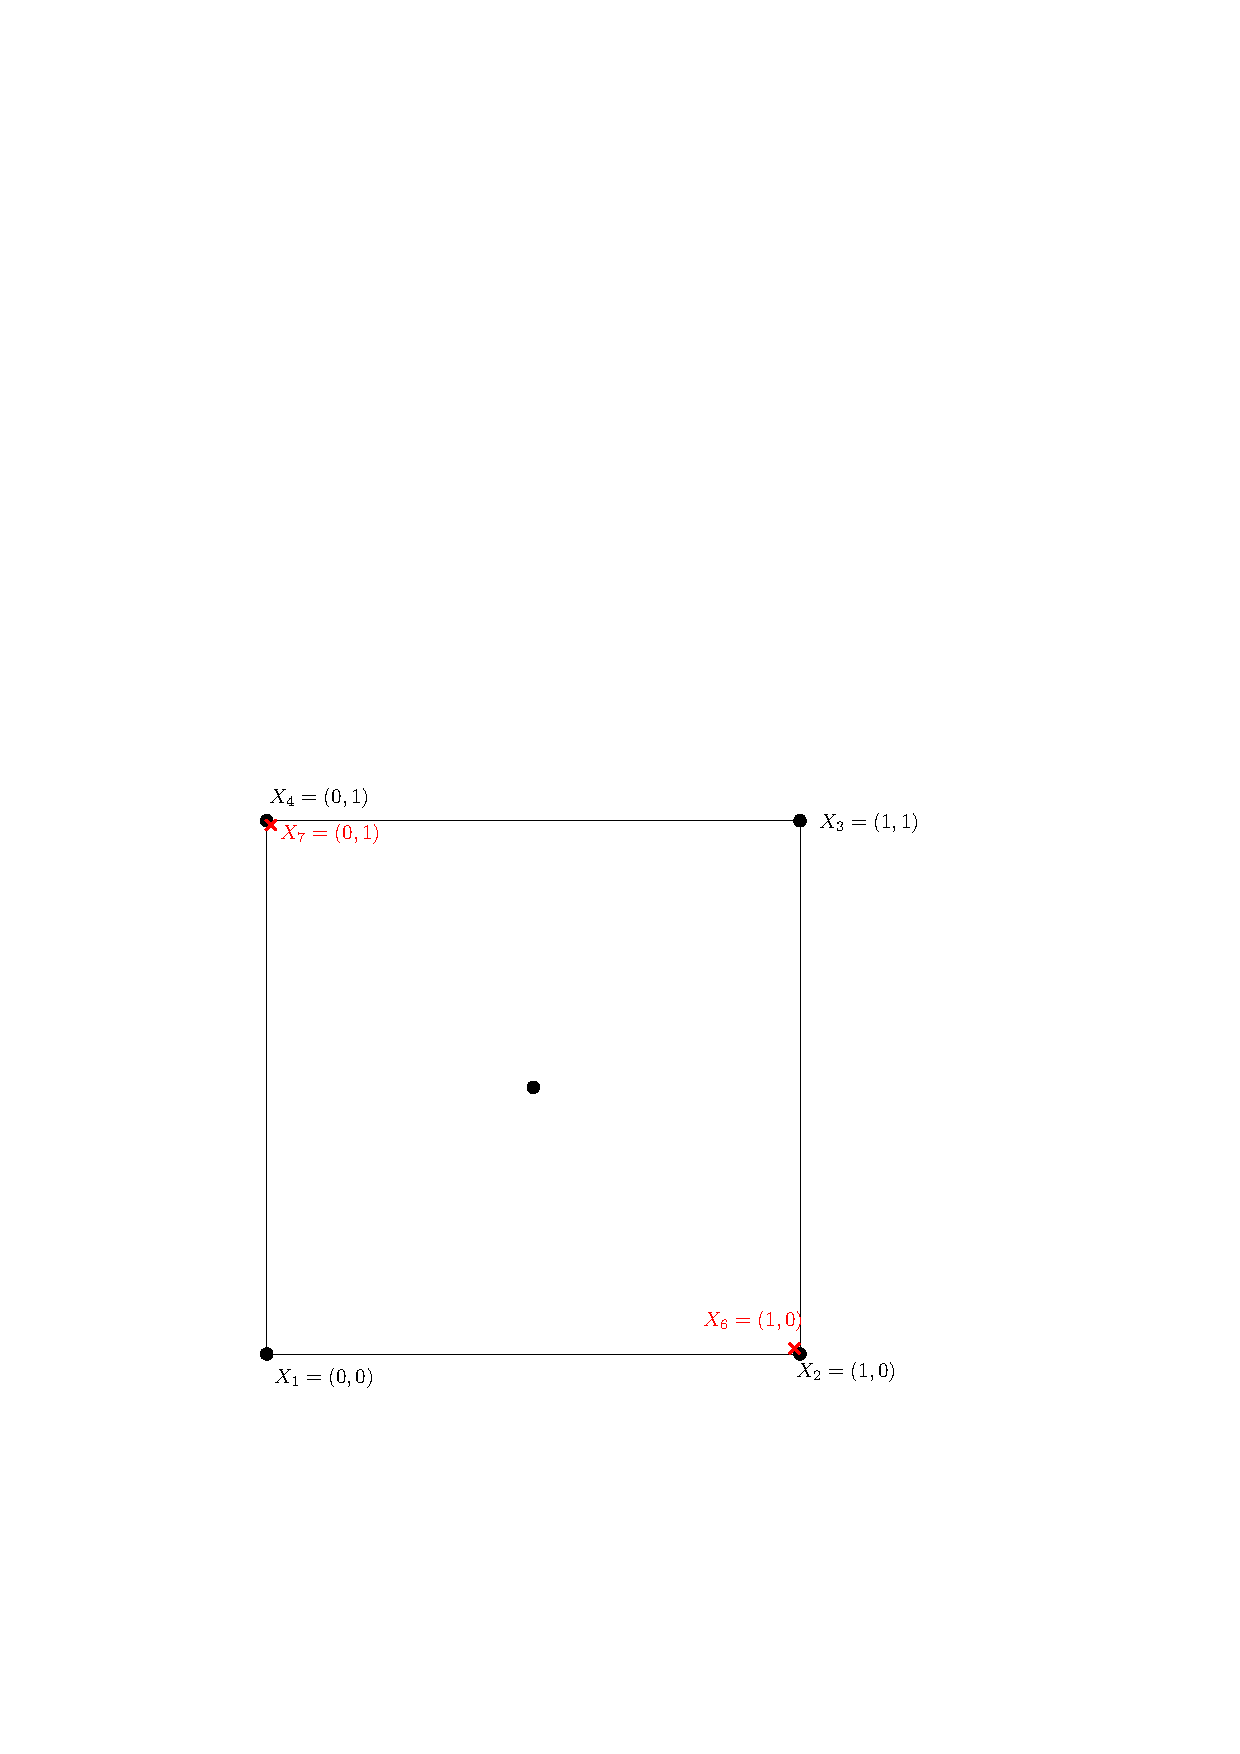
\includegraphics{multmin-diag}
 \end{figure} 
  Suppose $X_6$ is matched with $X_2$ and $X_7$ is matched with $X_4$. 
  Denote the Euclidean distance matrix by $D$. 
  Suppose, due to noise, or due to dissimilarities not being Euclidean distances, 
  our dissimilarity matrix is $$D'_{ij}=\begin{cases}
  D_ij-1.4 & \textrm{if  $(i,j) \in \{(4,6),(6,4),(2,7),(7,2)   \}$ }\\
  D_ij  & \textrm{ otherwise}\\
  \end{cases}.$$ 
Qualitatively, the three points $X_1$, $X_7$ and $X_3$ form a barrier which   the OOS points need to cross  to reach their matched counterparts.
   
   Based on the initial configuration, the  embedding coordinates of $\hat{X}_6$ might be closer
    to $X_4$ compared to $X_2$. This is due to a local minimum in the configuration space.  If $\hat{X}_6$ starts from the initial configuration where it's located on the $X_4$ side of the y=x line at the start of optimization, 
    it might have to cross paths with the embedding of  ${X}_1,{X}_3,{X}_7$ with which it has a  nonzero dissimilarity.  
    Based on value of $w$, it might be easier to get out of this local minimum. 
    In fact, depending on w can this  local minimum can be a global minimum. 
    That is, the configuration where $X_6$ stays on the side of $X_4$ instead of $X_2$ might have a lower stress than the configuration where $X_6$ is near $X_2$. 
    The following plots shows the local minimum $\hat{X}_6$ ends up in, depending on initial configuration. 
    Depending on $w$ value, one of these minima has a lower weighted stress than the other.   

\begin{figure}
\begin{minipage}[b]{0.5\linewidth}
\centering
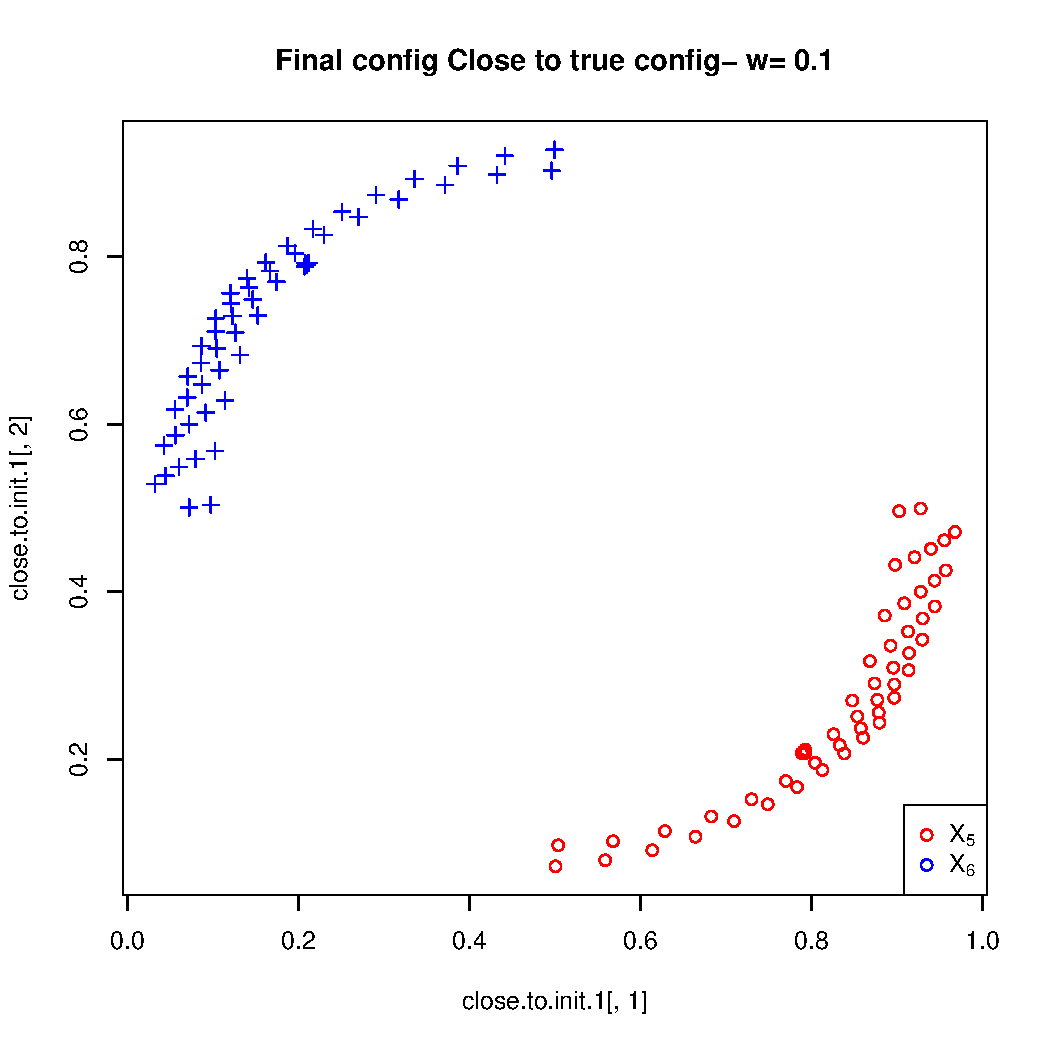
\includegraphics[scale=0.35]{true-min-w-0_1.pdf}

\label{fig:figure1-1}
\end{minipage}
\hspace{0.5cm}
\begin{minipage}[b]{0.5\linewidth}
\centering
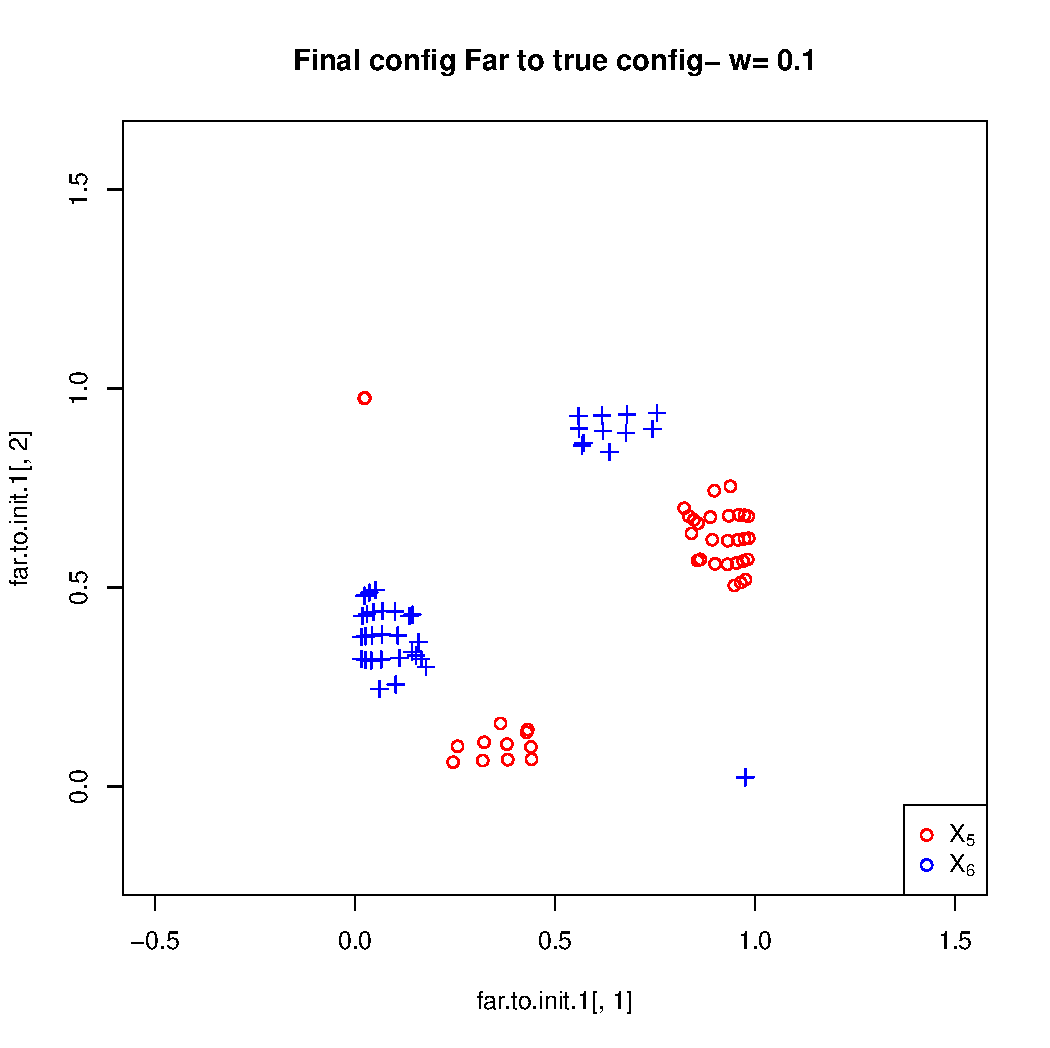
\includegraphics[scale=0.35]{other-min-w-0_1.pdf}

\label{fig:figure1-2}
\end{minipage}

\caption{Final configurations for for different $w=0.1$ }
\label{fig:Finalconfig-MultMin-w-0_1}

\end{figure}




\begin{figure}
\begin{minipage}[b]{0.5\linewidth}
\centering
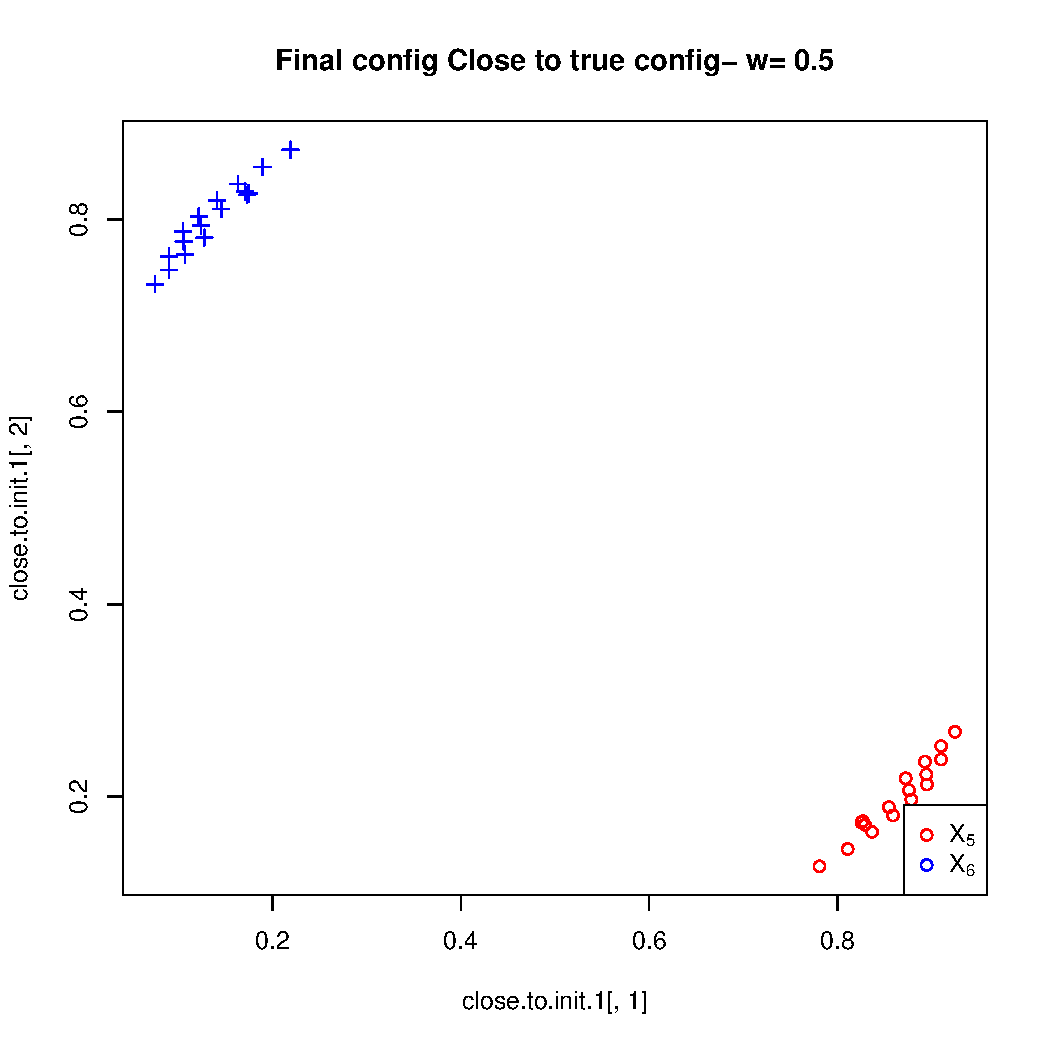
\includegraphics[scale=0.35]{true-min-w-0_5.pdf}

\label{fig:figure2-1}
\end{minipage}
\hspace{0.5cm}
\begin{minipage}[b]{0.5\linewidth}
\centering
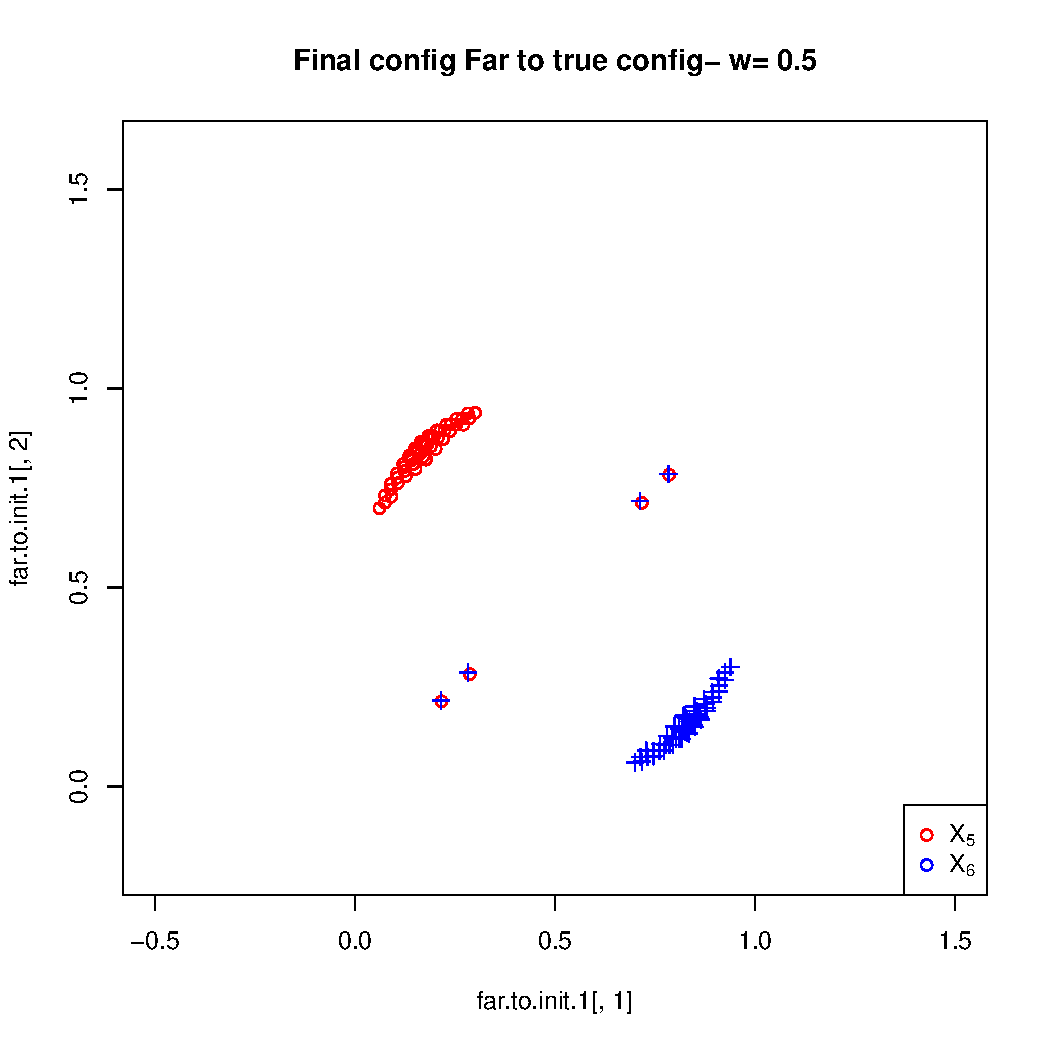
\includegraphics[scale=0.35]{other-min-w-0_5.pdf}

\label{fig:figure2-2}
\end{minipage}

\caption{Final configurations for for different $w=0.5$ }
\label{fig:Finalconfig-MultMin-w-0_5}

\end{figure}


\begin{figure}
\begin{minipage}[b]{0.5\linewidth}
\centering
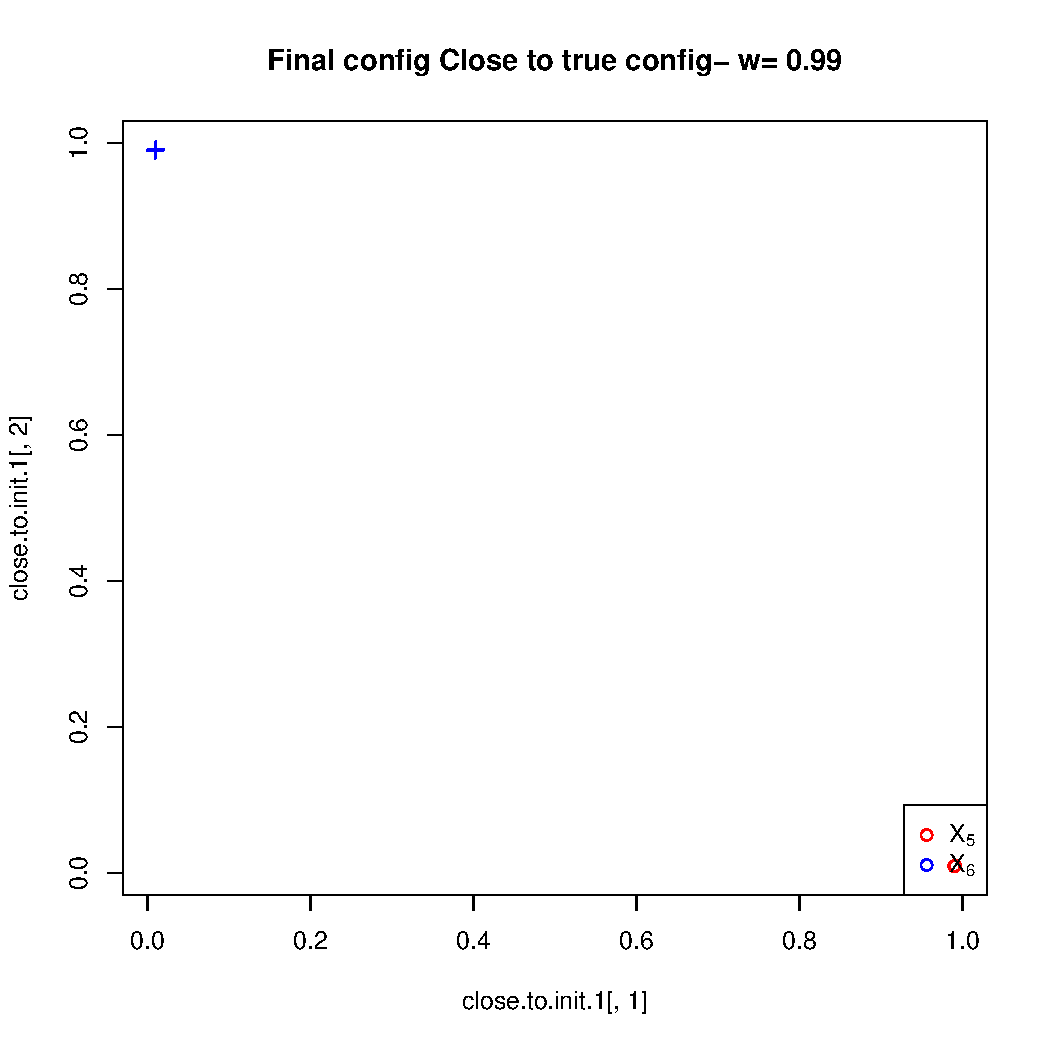
\includegraphics[scale=0.35]{true-min-w-0_99.pdf}

\label{fig:figure2-1}
\end{minipage}
\hspace{0.5cm}
\begin{minipage}[b]{0.5\linewidth}
\centering
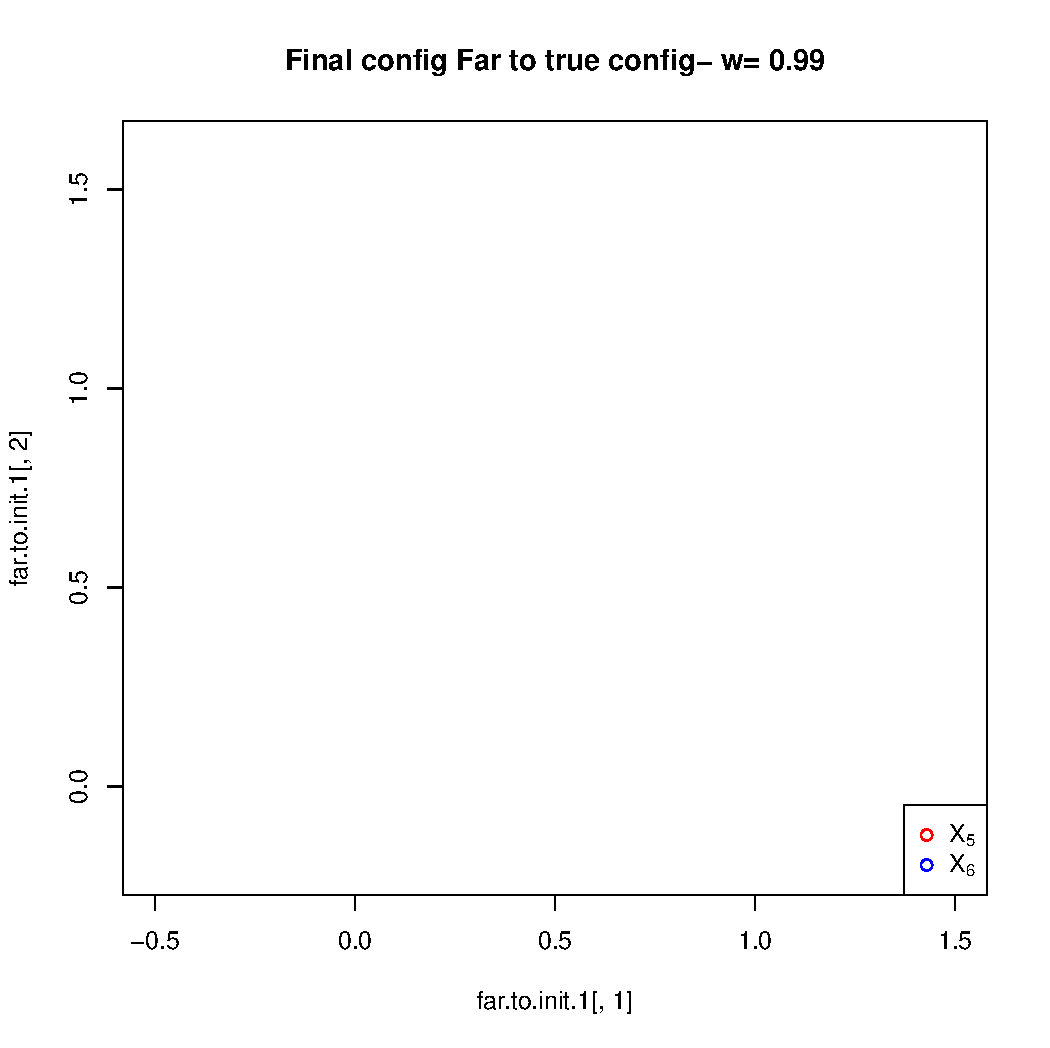
\includegraphics[scale=0.35]{other-min-w-0_99.pdf}

\label{fig:figure2-2}
\end{minipage}

\caption{Final configurations for for different $w=0.99$ }
\label{fig:Finalconfig-MultMin-w-0_99}

\end{figure}


\begin{table}[ht]
\begin{center}
\begin{tabular}{rrrrrr}
  \hline
 $w$ value & 0.1 & 0.45 & 0.5 & 0.55 & 0.99 \\ 
  \hline
Local min for real config. & 2.80 & 1.77 & 1.62 & 1.47 & 0.04 \\ 
  Alternative local min & 0.39 & 1.53 & 1.65 & 1.74 & 100.00 \\ 
   \hline
\end{tabular}
\end{center}
\end{table}

Other than such carefully constructed examples, we expect $w$ to have no effect on the ordering of the local minima according to their stress values.
Therefore,  the argmin among these local minima is independent of $w$. The minimum configuration is then a continuous function of $w$. 
By the continuity of the distance function with respect to configurations, the test statistic is continuous with respect to $w$. One can conclude $\beta(w) $ is a continuous function of $w$. 
%It is possible this is not the global minimum in $\mathbb{R}^d$  

%Does the discontinuity in configurations mean discontinuity  in the $\beta(w)$ function
%It is possible this is not the global minimum in $\mathbb{R}^d$  
 
\begin{comment}

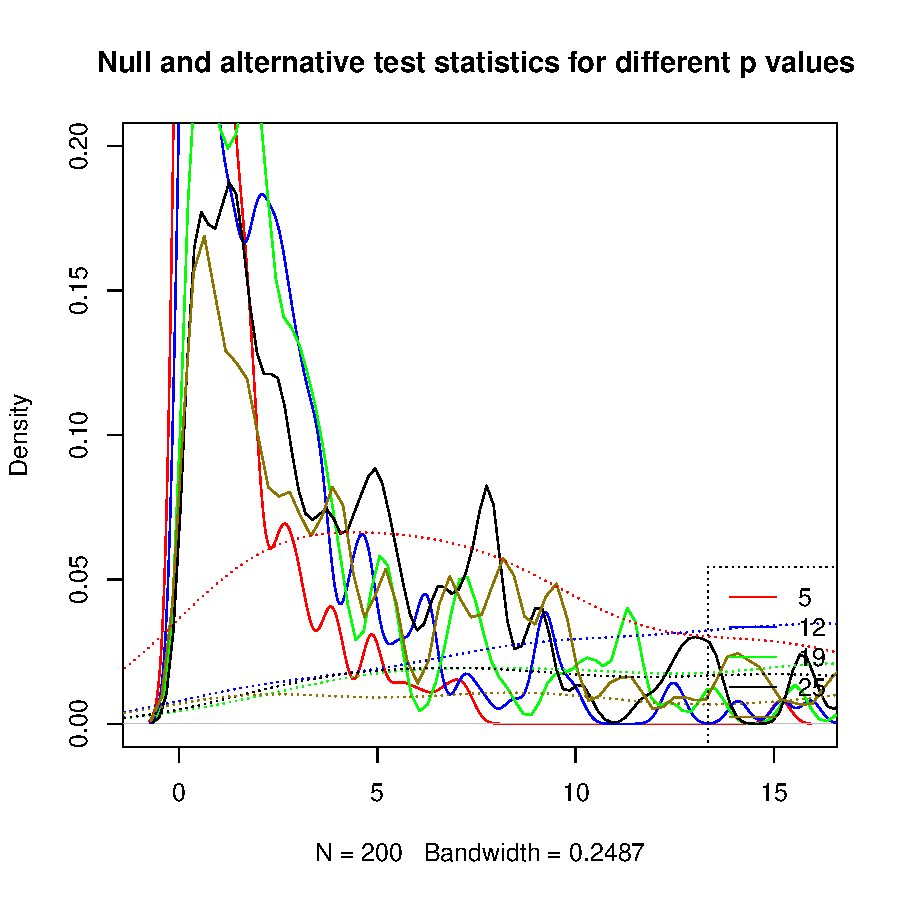
\includegraphics{FidCommPaper-fig-stats-p}



 , so any $w$ value that takes advantage of this situation and captures fidelity will limit the growth of the test statistic under alternative. So such $w$ values that are small enough to preserve fidelity, yet large enough to not lose significantly from commensurability will have increases in power to become $w^*$. 




Consider  an increase in $r$, this will cause the test statistic under null to be stochastically smaller,
 leading to a smaller critical value. So , a increase in priority of fidelity,
  which corresponds to smaller $w$ might lead to the increase in the test statistic under alternative, and therefore an increase in power.\ref{fig-stats-r}  



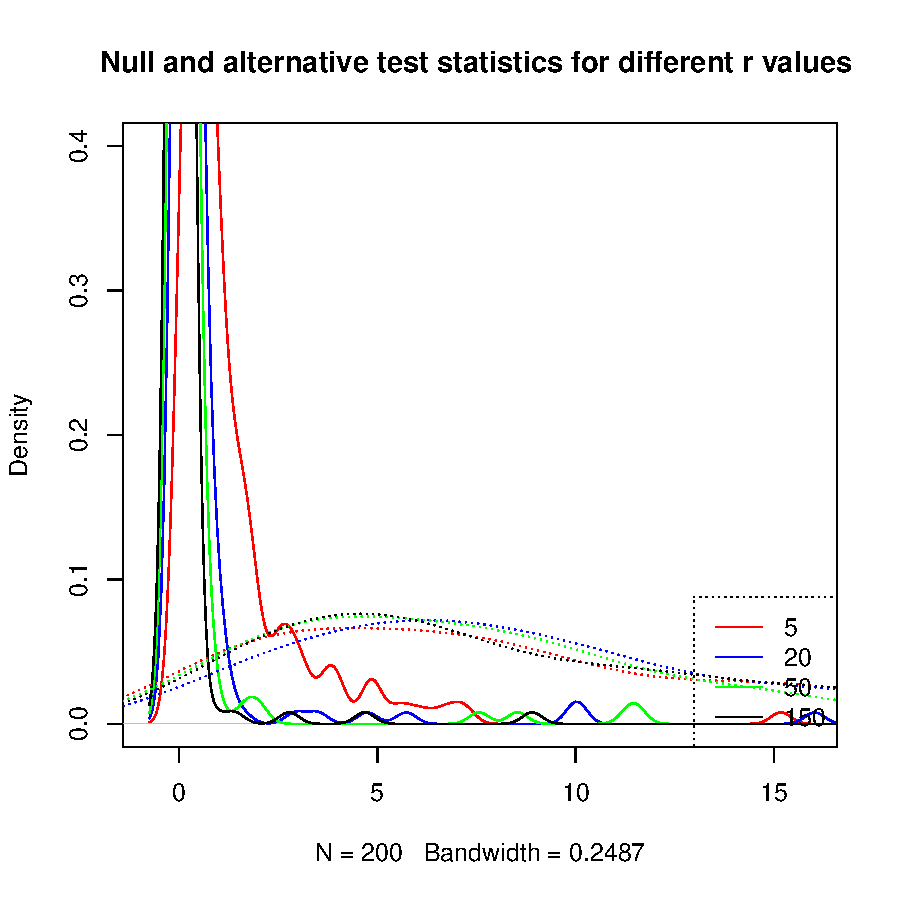
\includegraphics{FidCommPaper-fig-stats-r}

Consider increases in $c$, which will increase the dissimilarity  both between matched and between unmatched vectors. 



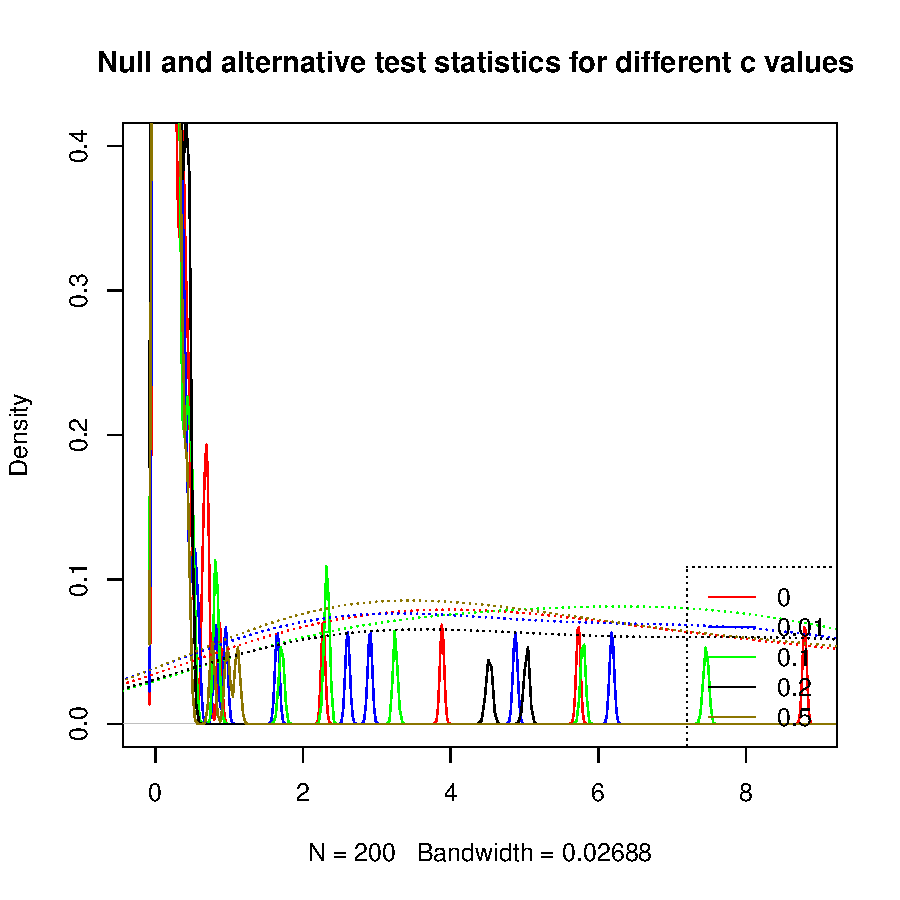
\includegraphics{FidCommPaper-fig-stats-c}




Consider increases in $q$,  the test statistic under both null and alternative is inflated\ref{fig-stats-q}. 


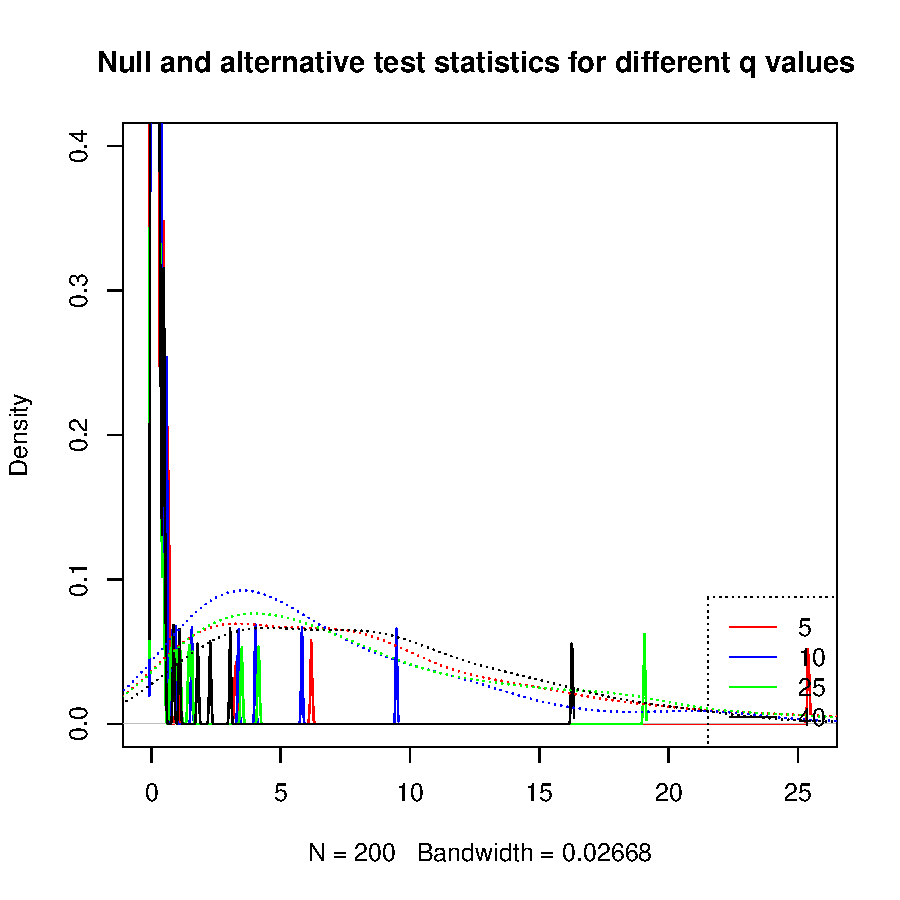
\includegraphics{FidCommPaper-fig-stats-q}
 If commensurability can be preserved in the face of the increase in $q$, the power of the test may be preserved. However a very large increase in $w$ is not guarenteed to increase the preservation of commensurability, since the extra dimensions are noise, trying to   make the differences between coordinates  small in those dimensions will not  help in power, in fact may be disruptive since,
  more fidelity may be lost in the effort to bring the pair of points together.

\end{comment}




\section{Simulation Results\label{sec:Simulation Results}}
To compare the  different approaches, training data of matched sets of measurements were generated according to the Dirichlet and Gaussian settings. Dissimilarity representations were generated from pairwise distances of measurements. A set of matched pairs of measurements and unmatched pairs of measurements were also generated for testing. The test statistics (computed via P$\circ $M, CCA and JOFC approaches) for matched and unmatched pairs were used to compute power values at a set of fixed type I error rate $\alpha$ values.

 Additionally, to take robustness of methods into consideration, ``noisy" measurements were created from the original measurements by concatenating randomly generated independent noise vectors (subsection \ref{noise}).   This setting will be referred to as the ``noisy case". The original setting, with $c=0$,  will be referred as the ``noiseless case".
If the magnitude of noise (controlled by the parameter $c$ in equation \eqref{eq:noise-expr}) is small enough, PCA and MDS will not be affected significantly, but if the number of noisy dimensions (controlled by the parameter $q$ in the distribution of $E_{ik}$ as defined in equation \eqref{eq:noise-expr}) is large enough, CCA  will be affected due to spurious correlation between noisy dimensions.

Given the setting ("Gaussian","Dirichlet"),   the steps for each Monte Carlo replicate are as follows:
\begin{itemize}
\item A training set ($\mathbf{T}_{mc}$) which consists of  $n$ pairs of matched measurements is generated.  If $c=0$, we are in the ``noiseless" setting and measurements are $p$-dimensional vectors, otherwise we are in the ``noisy" setting and measurement vectors are $(p+q)$-dimensional.
\item Dissimilarities are computed and embedded in  Euclidean space  via MDS (followed by a transformation from  $\mathbf{R}^d$ to  $\mathbf{R}^d$ and  projection into $\mathbf{R}^d$, respectively  for P$\circ$M and CCA) . The final embeddings lie in $\mathbb{R}^d$.   Denote this in-sample embedding as   $\hat{\mathbf{T}}$. Note that  if the JOFC method is being used, embedding is carried out with the weighted raw stress function $\sigma_{W}(\cdot)=f_{w}(D(\cdot),M)$ in equation \eqref{fid-comm-tradeoff-func} with a common weight $w$ for commensurability terms and another common weight $1-w$ for fidelity terms, otherwise unweighted raw stress function ($\sigma(\cdot)$) is used as a criterion function for embedding.

\item We generate $m$ pairs of matched   measurements  which we treat as out-of-sample, and 
\begin{itemize}
\item compute the dissimilarities  %$\mathbf{\Delta}^{new}={ \delta_{ik}^{new}; i=1,\ldots, n;\hspace{5pt} k=1,2}$
 between these out-of-sample  points and the points in ${\mathbf{T}_{mc}}$,  
\item  embed the OOS dissimilarities as pairs of embedded points via the OOS extension:\\
 $(\tilde{y}_1^{(1)},\tilde{y}_1^{(2)}),\ldots, (\tilde{y}_m^{(1)},\tilde{y}_m^{(2)})$, 
\item compute the test statistic $\tau$ for each pair.%, $t(\tilde{y}_i^{(1)},\tilde{y}_i^{(2)});\hspace{4pt}
%i=1,\ldots,m$
\end{itemize}
 The values of the statistic $\tau$ are used for computing  the empirical cumulative distribution function under null hypothesis. 

\item Identical steps for $m$ pairs of unmatched measurements result in the empirical cumulative distribution  function of $\tau$ under alternative hypothesis.
\item For any fixed $\alpha$ value, a critical value for the test statistic and the corresponding power is computed.
\end{itemize}






\begin{figure}
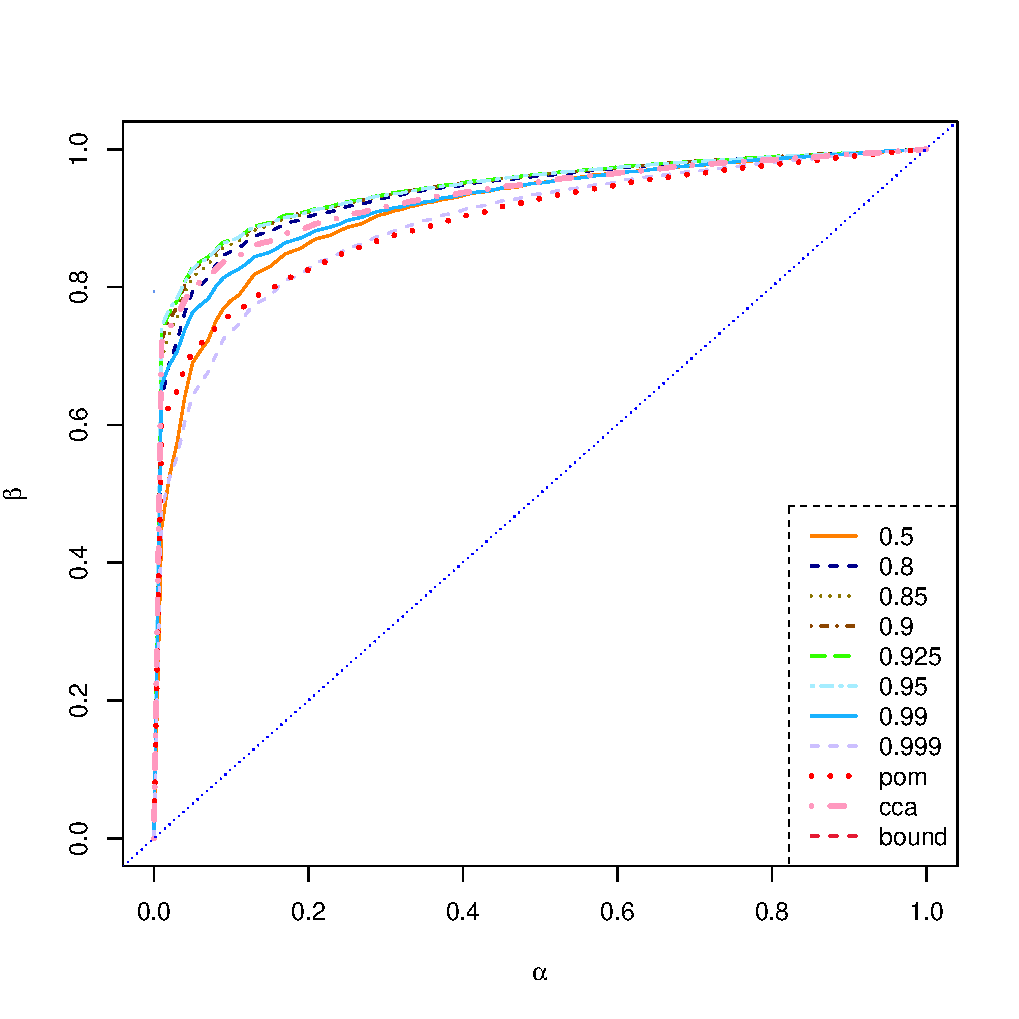
\includegraphics[scale=0.35]{MVN-FC-Tradeoff-OOSc0-01-n150.pdf}
\caption{Power ($\beta$) vs Type I error ($\alpha$) plot for different $w$ values for the Gaussian setting (noisy case)}
\label{fig:MVN-c001-power-alpha}
\end{figure}

\begin{figure}
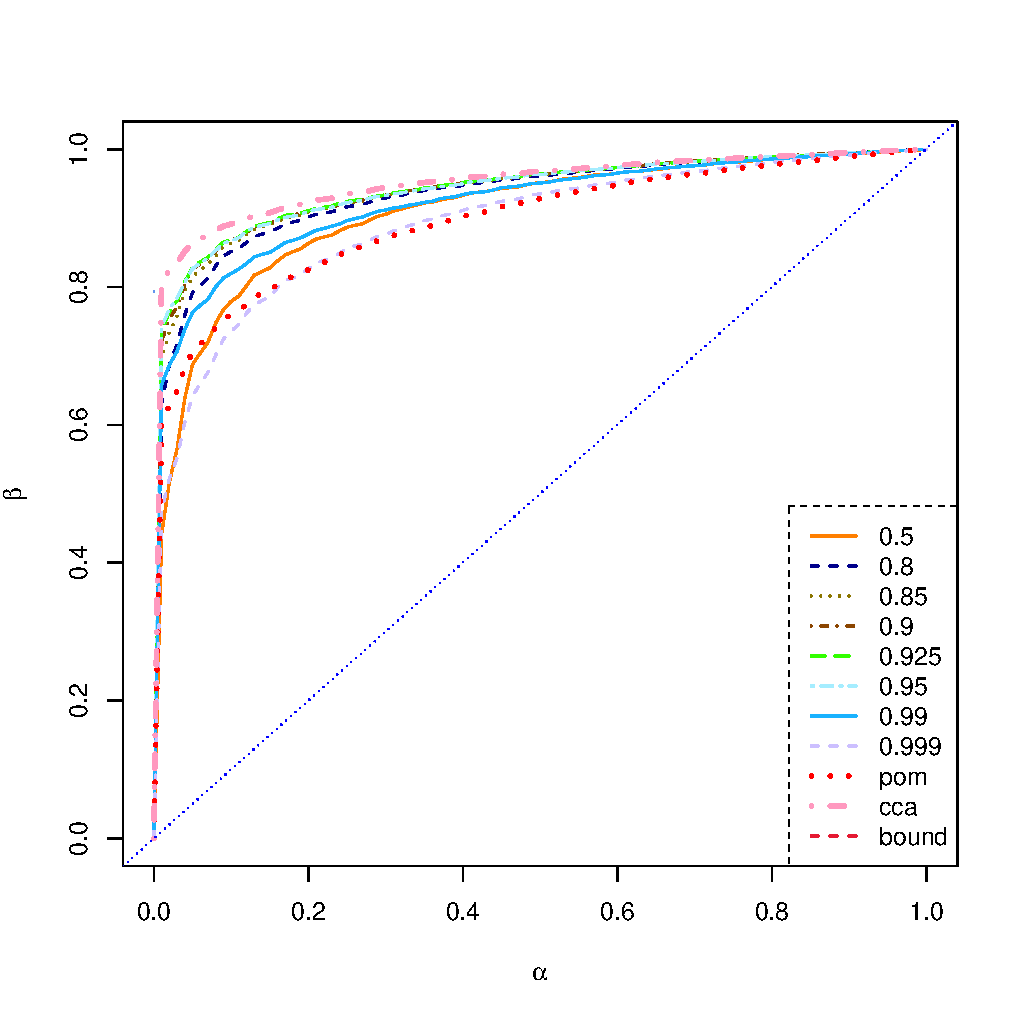
\includegraphics[scale=0.35]{MVN-FC-Tradeoff-OOSc0-n150.pdf}
\caption{Power ($\beta$) vs Type I error ($\alpha$) plot for different $w$ values for the Gaussian setting (noiseless case)}
\label{fig:MVN-c0-power-alpha}
\end{figure}

\begin{figure}
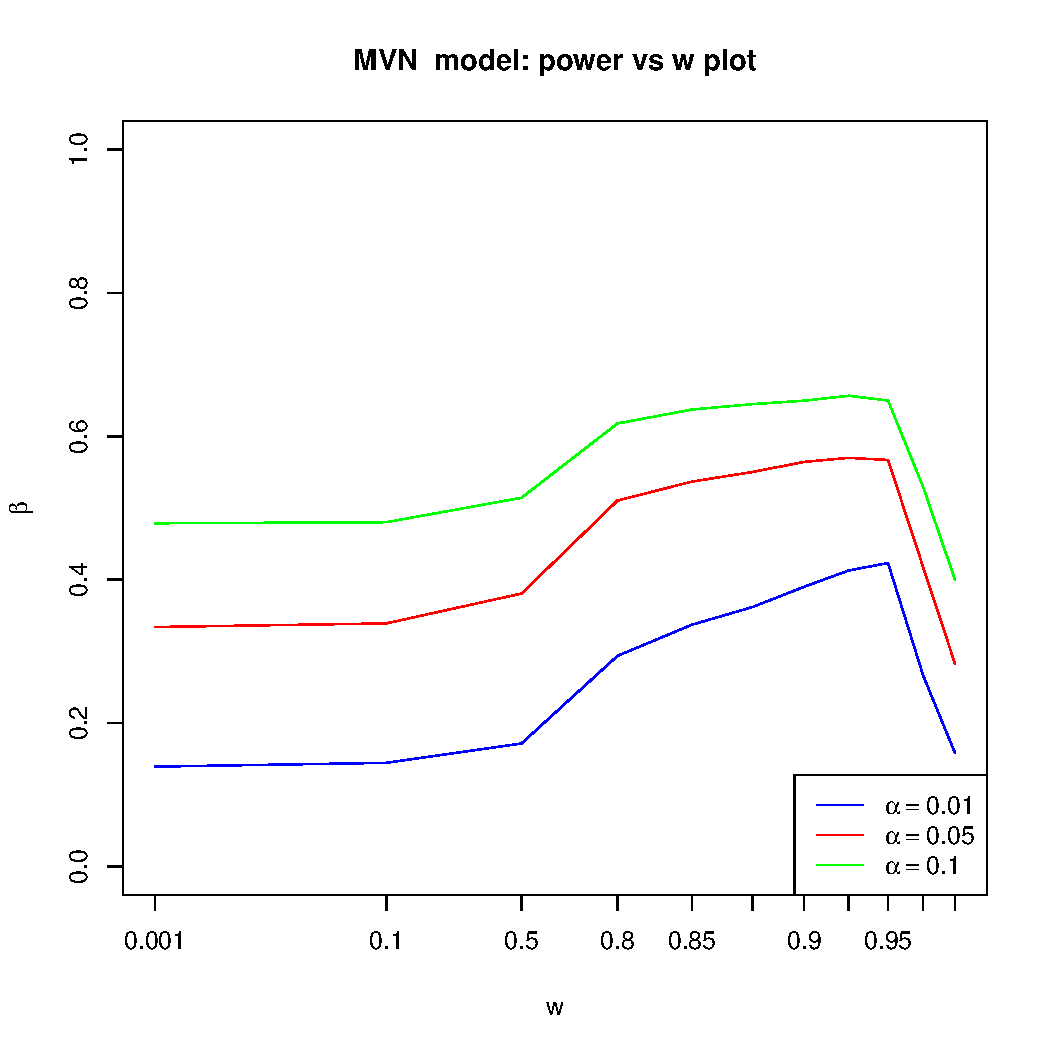
\includegraphics[scale=0.95]{OOS-MVN-power-w-c0-01.pdf}
\caption{Power ($\beta$) vs $w$ plot for different Type I error ($\alpha$) values for the Gaussian setting (noisy case)}
\label{fig:MVN-c001-power-w}
\end{figure}


\begin{figure}
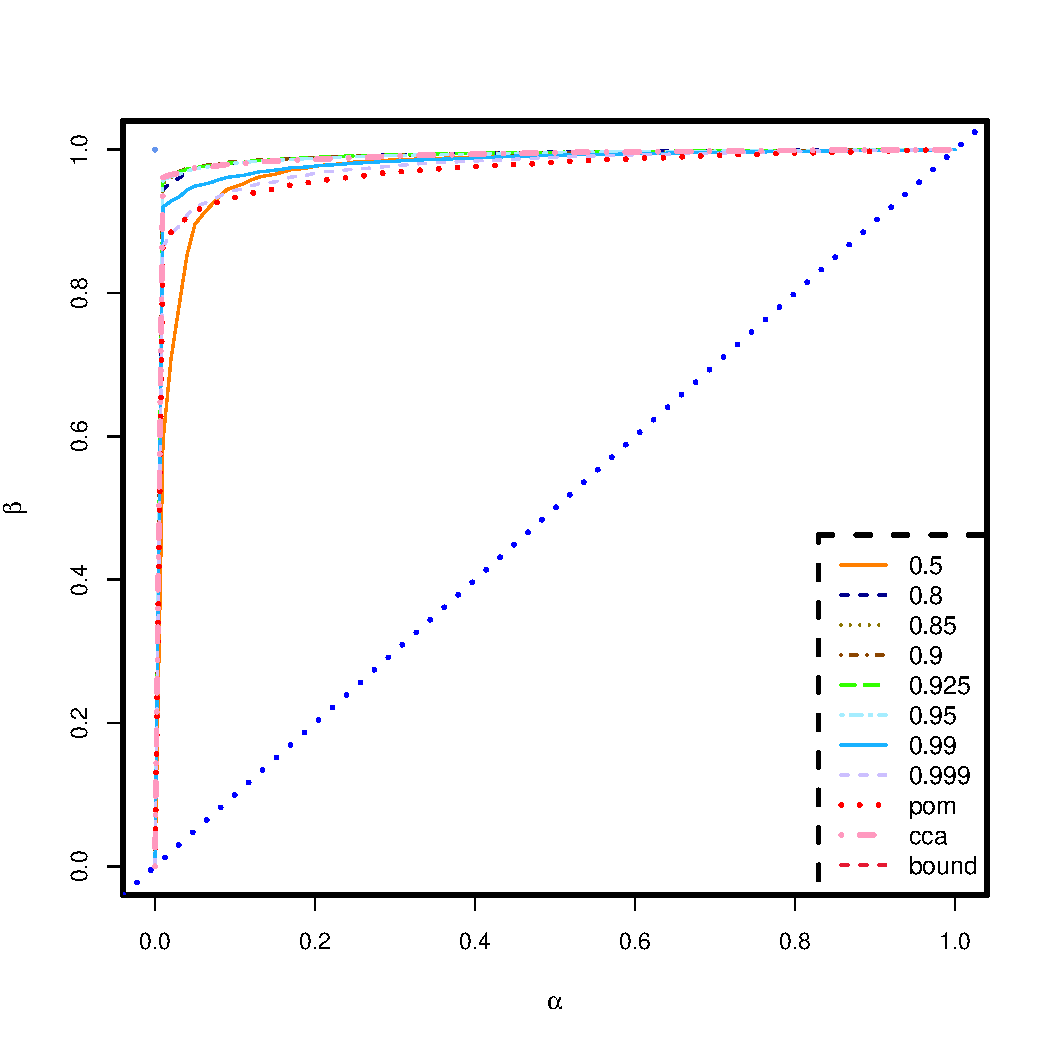
\includegraphics[scale=0.35]{Dirichlet-FC-Tradeoff-OOSc0-01-n150.pdf}
\caption{Power ($\beta$) vs Type I error ($\alpha$) plot for different $w$ values for the Dirichlet setting (noisy case)}
\label{fig:Dir-c001-power-alpha}
\end{figure}

\begin{figure}
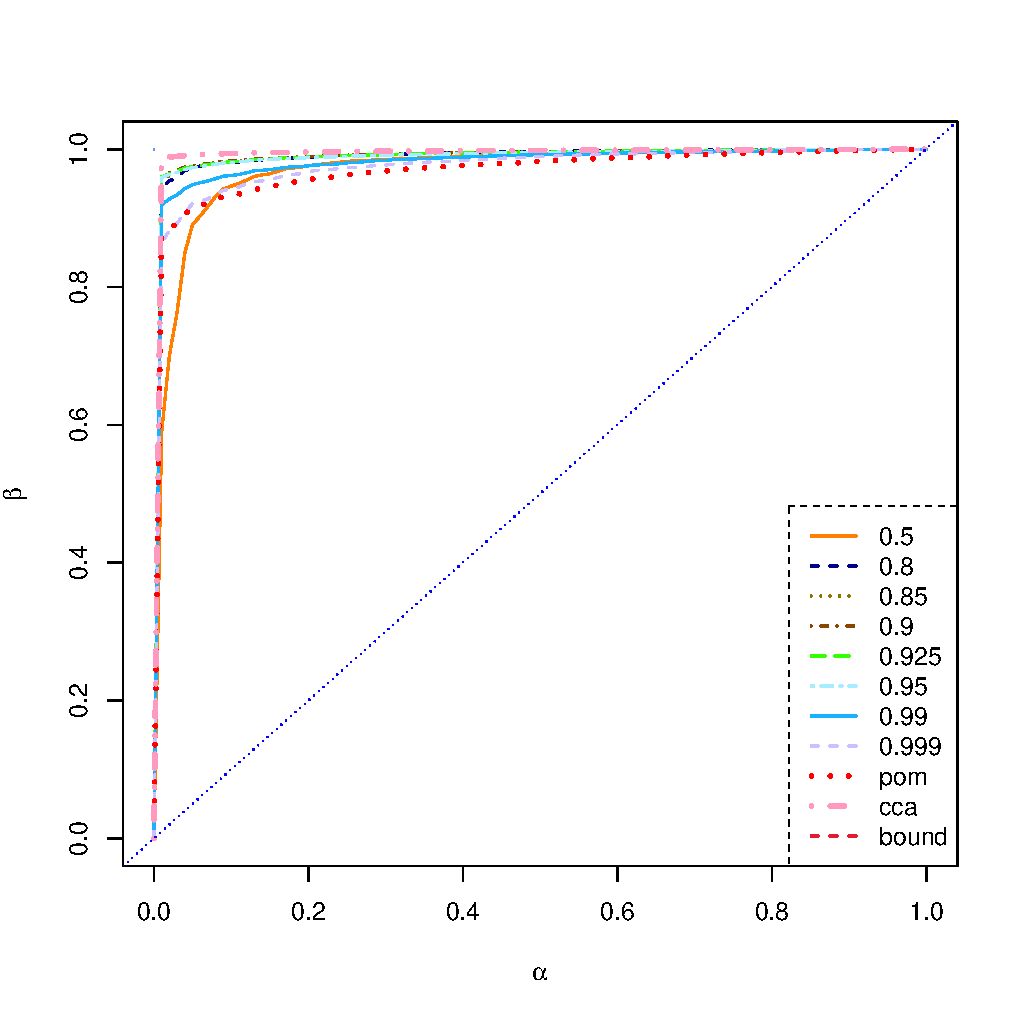
\includegraphics[scale=0.35]{Dirichlet-FC-Tradeoff-OOSc0-n150.pdf}
\caption{Power ($\beta$) vs Type I error ($\alpha$) plot for different $w$ values for the Dirichlet setting (noiseless case)}
\label{fig:Dir-c0-power-alpha}
\end{figure}

\begin{figure}
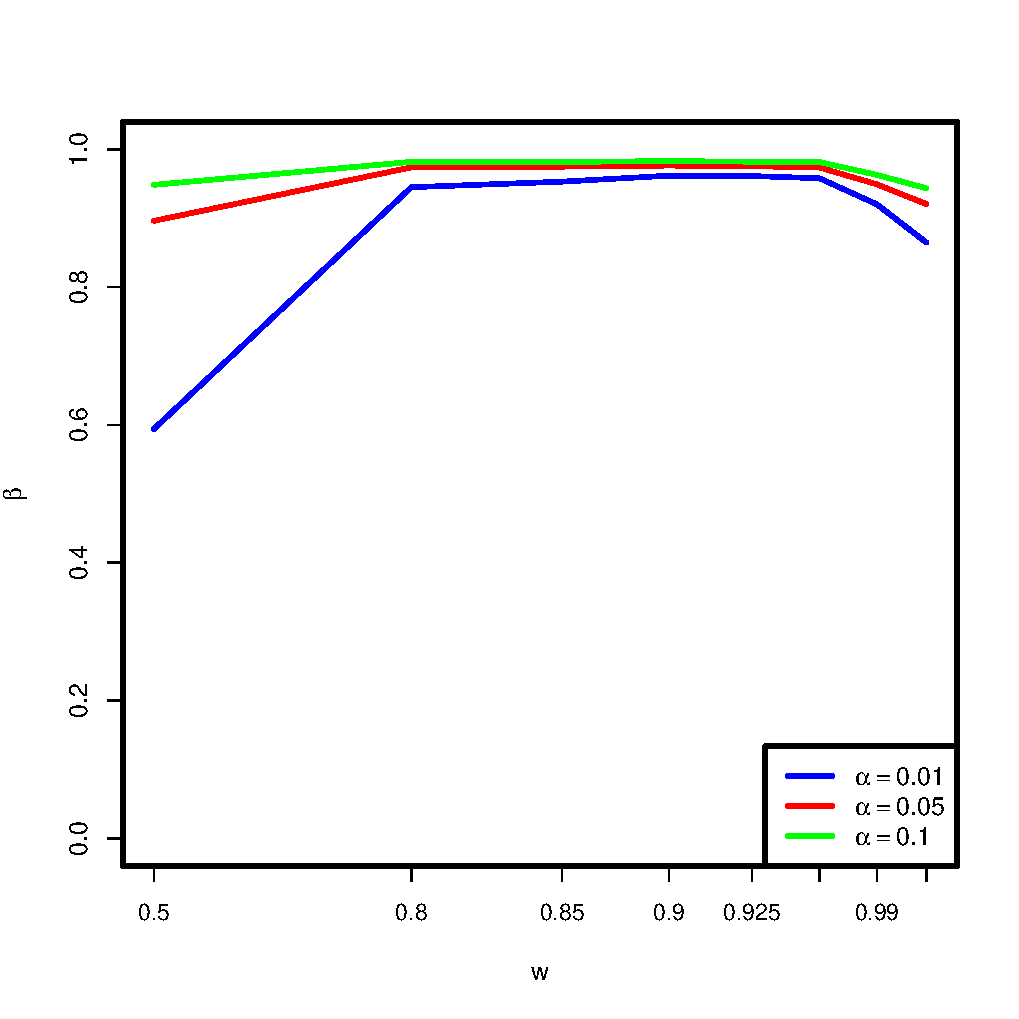
\includegraphics[scale=0.95]{OOSDirichlet-power-w-c0-01.pdf}
\caption{Power ($\beta$) vs $w$ plot for different Type I error ($\alpha$) values for the Gaussian setting (noisy case)}
\label{fig:MVN-c001-power-w}
\end{figure}

Setting p and q to 5 and 10, respectively, for $n=150$ and $m=150$, the average of the power values for $nmc=150$ Monte Carlo replicates are computed at  different $\alpha$s and are plotted in Figure \ref{fig:MVN-c001-power-w} against $\alpha$ for the Gaussian setting.  Qualititatively similar plots for the Dirichlet setting  exist.  The plot in Figure \ref{fig:MVN-c001-power-w} shows that for different values of  $w$, we have varying power curves, and some $w$ values outperform others in terms of power. In Figure \ref{fig:MVN-c001-beta-w},  $\beta(w)$ is plotted against $w$ for fixed values of $\alpha$. It is  interesting that the optimal value of $w$ seems to be in the range of $(0.85,1)$ for all settings, which suggests commensurability might be more critical for our hypothesis testing task. 




\begin{comment}
\begin{figure}
\includegraphics[scale=0.35]{OOS-MVN-power-w-c0.pdf}
\caption{$\beta$ vs $w$ plot for fixed $\alpha$ values for the Gaussian setting (noiseless case)}
\label{fig:MVN-c0-beta-w}
\end{figure}
\end{comment}

\begin{figure}
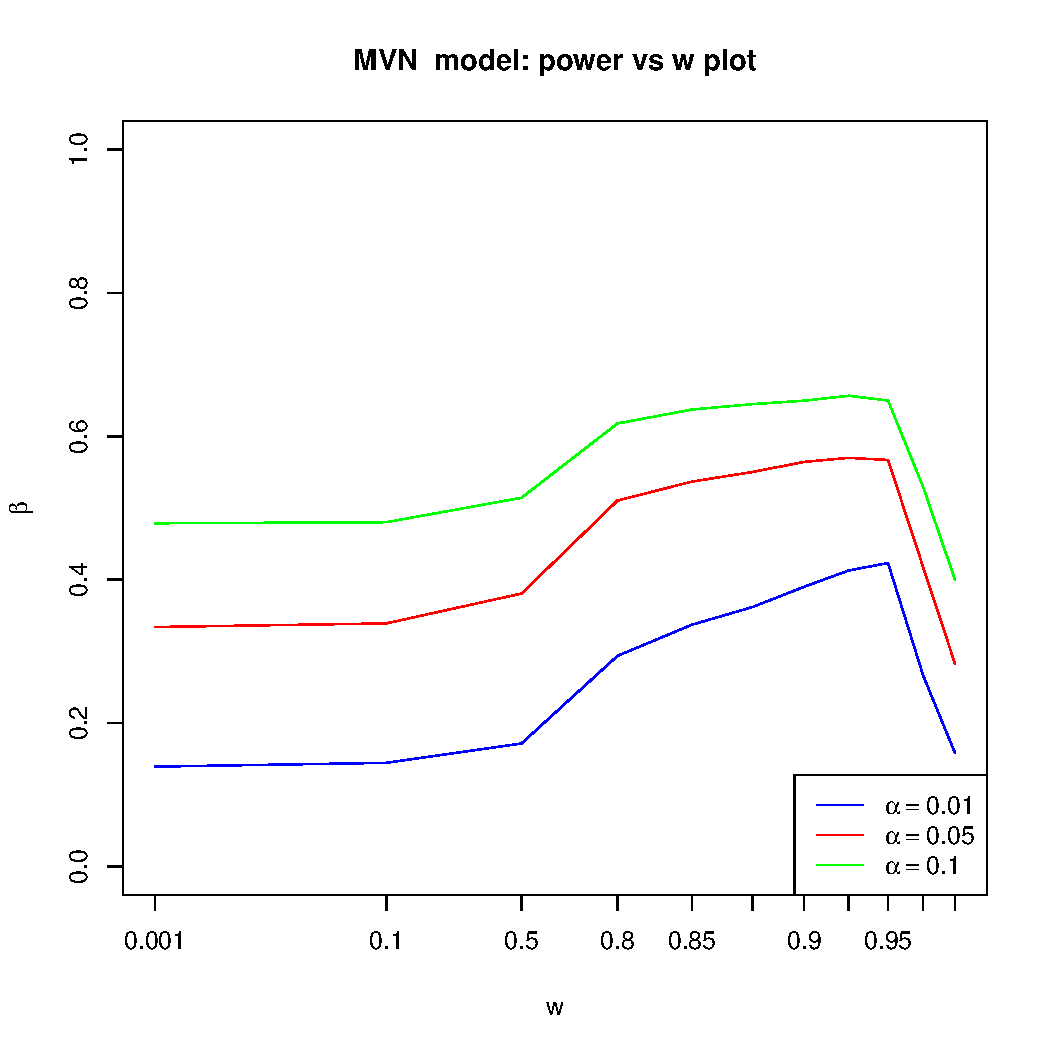
\includegraphics[scale=0.65]{OOSMVN-power-w-c001.pdf}
\caption{Power ($\beta$) vs $w$ plot for fixed Type I error ($\alpha$) values for the Gaussian setting (noisy case)}
\label{fig:MVN-c001-beta-w}
\end{figure}
Note that in Figure \ref{fig:MVN-c001-beta-w} for $\alpha=0.05$, $\beta_{\alpha=0.05}(w=0.99)\geq\beta_{\alpha=0.05}(w=0.5)$. However, for $\alpha=0.2$, $\beta_{\alpha=0.2}(w=0.99)\leq\beta_{\alpha=0.2}(w=0.5)$. This justifies our comment that  $w^{*}$  must be defined with respect to $\alpha$.


\begin{comment}
\begin{figure}
\includegraphics[scale=0.35]{OOS-Dirichlet-power-w-c0.pdf}
\caption{$\beta$ vs $w$ plot for fixed $\alpha$ values for the Dirichlet setting(noiseless case)}
\label{fig:fig7}
\end{figure}

\begin{figure}
\includegraphics[scale=0.35]{OOS-Dirichlet-power-w-c0-01.pdf}
\caption{$\beta$ vs $w$ plot for fixed $\alpha$ values for the Dirichlet setting(noisy case)}
\label{fig:fig8}
\end{figure}
\end{comment}



Note that  for all of the settings, the estimate of the optimal $w^{*}$ has  higher power than $w$=0.5 (the unweighted case).
To test the statistical significance of this observation, we wish to test the null hypothesis that  $H_{0}: \beta_{\alpha}({\hat{w}^*})\leq\beta_{\alpha}({w=0.5})$ against the alternative $H_{A}=\beta_{\alpha}({\hat{w}^*})>\beta_{\alpha}({w=0.5})$.  The least favorable null hypothesis is that  $H_{0}: \beta_{\alpha}({\hat{w}^*})=\beta_{\alpha}({w=0.5})$.

For a fixed $\alpha$ value, one can compute two critical values  using the test statistic values for the two $w$ values that are being compared. Using these critical  values, we can  determine the decision made by each test for each pair of embedded points, $(\tilde{y}_i^{(1)},\tilde{y}_i^{(2)}),\hspace{7pt}i=1,\ldots,m$. To compare the  two statistical tests with different $w$ values, one can prepare a $2\times 2$ contingency-table of correct decisions and incorrect decisions made by each statistical test (or equivalently true and false classifications made by two classifiers). Denote decision outcome as $c_1$ for the first statistical test and $c_2$ for the second statistical test. If $c_1=True$ and $c_2=False$ for an instance,  the first test made the correct decision and the second test made the incorrect decision with regard to the null and alternative hypotheses.
% McNemar's test was used to compare the two contingency tables for fixed $\alpha$. McNemar's test is a statistical test for %comparing two binary classifiers based on a 2-by-2 table of the counts of misclassifications of each. That is,
Consider the contingency table for a Monte Carlo replicate given by $$G^{(l)}= \begin{array}{|c|c|}
      \hline
       e_{FF}^{(l)} & e_{TF}^{(l)}\\
      \hline
       e_{FT}^{(l)} & e_{TT}^{(l)}\\
      \hline
      \end{array}      $$  where $l$ is the index of the MC replicate, $e_{c_1c_2}^{(l)}$ is equal to the number of instances at which the true hypothesis were identified  correctly ($c_1=True$) or incorrectly ($c_1=False$) by the first test, and correctly ($c_2=True$) or incorrectly ($c_2=False$) by the second test in that MC replicate.

Under the null  hypothesis, $Pr[\left(c_1c_2\right)=(TF)]=Pr[\left(c_1c_2\right)=(FT)]$, so $\sum_l{I \{e_{TF}^{(l)}>e_{FT}^{(l)}\}}$ will be distributed according to  the binomial distribution, $\mathcal{B}(nmc,0.5)$. ($I\{\cdot\}$ is the indicator function.) 

% For each Monte Carlo replicate, the p-value of McNemar's test was computed separately.

\begin{comment}
\begin{figure}
\begin{tabular}{p{4.7cm}p{4.7cm}}
$e_{00}$:Misclassified by \newline Both C1 and C2 & $e_{10}$:Correctly Classified by C1,\newline Misclassified by C2\\
& \\
$e_{01}$:Correctly Classified by C1, \newline Misclassified by C2 & $e_{11}$:Correctly Classified by \newline Both C1 and C2
\end{tabular}. 

\caption{Contingency Table for McNemar's test for comparing two classifiers, C1 and C2}
\label{fig:cont-table}
\end{figure}
\end{comment}

For the noisy version of the Gaussian setting at allowable type I error 0.05 for the two tests, when comparing  the null hypothesis that  $H_{0}: \beta_{\alpha}({\hat{w}^*})=\beta_{\alpha}({w=0.5})$ against the alternative $H_{A}=\beta_{\alpha}({\hat{w}^*})>\beta_{\alpha}({w=0.5})$, we find $p<1.09E-24$ which indicates the power using estimate of optimal $w^*$ is significantly greater than the power when using $w=0.5$. 
%In fact
% the distribution of p-values from McNemar's tests is skewed and  we reject $\beta_{0.5}>=\beta_{w^*} $ for  55\%  of the %Monte Carlo replicates.





Setting p and q to 5 and 10, respectively, for $n=150$ and $m=150$, the average of the power values for $nmc=150$ Monte Carlo replicates are computed at  different $\alpha$s and are plotted in Figure \ref{fig:MVN-c001-power-w} against $\alpha$ for the Gaussian setting.  Qualititatively similar plots for the Dirichlet setting  exist.  The plot in Figure \ref{fig:MVN-c001-power-w} shows that for different values of  $w$, we have varying power curves, and some $w$ values outperform others in terms of power. In Figure \ref{fig:MVN-c001-beta-w},  $\beta(w)$ is plotted against $w$ for fixed values of $\alpha$. It is  interesting that the optimal value of $w$ seems to be in the range of $(0.85,1)$ for all settings, which suggests commensurability might be more critical for our hypothesis testing task. 


\section{The general case of more than two conditions}


As it was mentioned, all of the approaches are generalizable to $K>2$ conditions, though some ambiguities need to be resolved. For example,  the alternative hypothesis could be  defined as the event that at least one of the K new dissimilarities are pairwise unmatched ($ H_{A1}: \exists i, j , 1\leq i < j \leq K :\bm{y}_{i} \nsim \bm{y}_{j} $ ) or it could be defined as the case that absolutely none of the K dissimilarities are matched   ($H_{A2}: \forall i, j , 1\leq i < j \leq K :\bm{y}_{i} \nsim \bm{y}_{j}$ )  .
% and the sample from the alternative must be generated accordingly during Monte Carlo simulation. In the first case, an appropriate test statistic is then the maximum of the pairwise %distances between embeddings of each test K-tuple.

For PoM, one can use Procrustes analysis  generalized to more than two configurations. Generalized Procrustes Analysis \cite{GPCA} is a well established method for finding a collection of linear transformations that minimizes the mismatch between the transformed configurations and a "mean`` shape computed from these configurations. 

For CCA, there are multiple generalizations available as the correlation between more than two configurations can be defined in multiple ways \cite{generalCCA}. Let $X_1,\ldots,X_K$ be random vectors. Consider the first set of canonical variates to be computed, $Z_1^{1},\ldots,Z_K^{1}$. Denote  the correlation matrix of  $Z_1^{1},\ldots,Z_K^{1}$ by $\Phi^{(1)}$.   The following three criteria  are proposed in \cite{generalCCA}.
\begin{itemize}
\item SUMCOR. Maximize the sum of the elements of $\Phi^{(1)}$ : $\mathbf{1'}(\Phi^{(1)})\mathbf{1'}$
\item MAXVAR. Maximize the largest eigenvalue of $\Phi^{(1)}$ : $\lambda^{(1)}_1$ 
\item  MINVAR. Minimize  the smallest eigenvalue of $\Phi^{(1)}$ : $\lambda^{(m)}_1$ 
\end{itemize}
One can think of all of these criteria as different norms on the correlation matrix.
%For $H_{A1}$ MINVAR might be a good choice, since the exploitation task is to find evidence against the null and as favorable to the alternative as possible. 
%MINVAR should be small whenever there exists \emph{at least} one unmatched measurement so under the alternative hypothesis. MAXVAR, in this case, wouldn't be necessarily small under alternative with respect to null.  MINVAR statistic should be stochastically smaller compared to null distribution. For $H_{A2}$ MAXVAR is appropriate, since under the alternative hypothesis, MAXVAR should be very small compared to under the null hypothesis. 
%For $H_{A2}$ MAXVAR is appropriate, since under the alternative hypothesis, MAXVAR should be very small compared to under the null hypothesis. It is quite possible the other generalizations are appropriate for our task.
An interesting question is whether any of these generalizations is more appropriate for $H_{A1}$ or $H_{A2}$.

A multivariate normal model with $K=3$ conditions were used to generate $K$-condition matched data. 
The simulations in the previous section\ref{sec:Simulation Results} were repeated with this $K$-condition data. 
The alternative was chosen as $ H_{A1}$ and SUMCOR was chosen as the generalization of CCA.
 $q$-dimensional noise vectors of magnitude $c$ were added to the matched measurements. 
 The ROC curves for these simulations are shown in \ref{fig:MVN-c001-power-w-Kcond}.


 

\begin{figure}
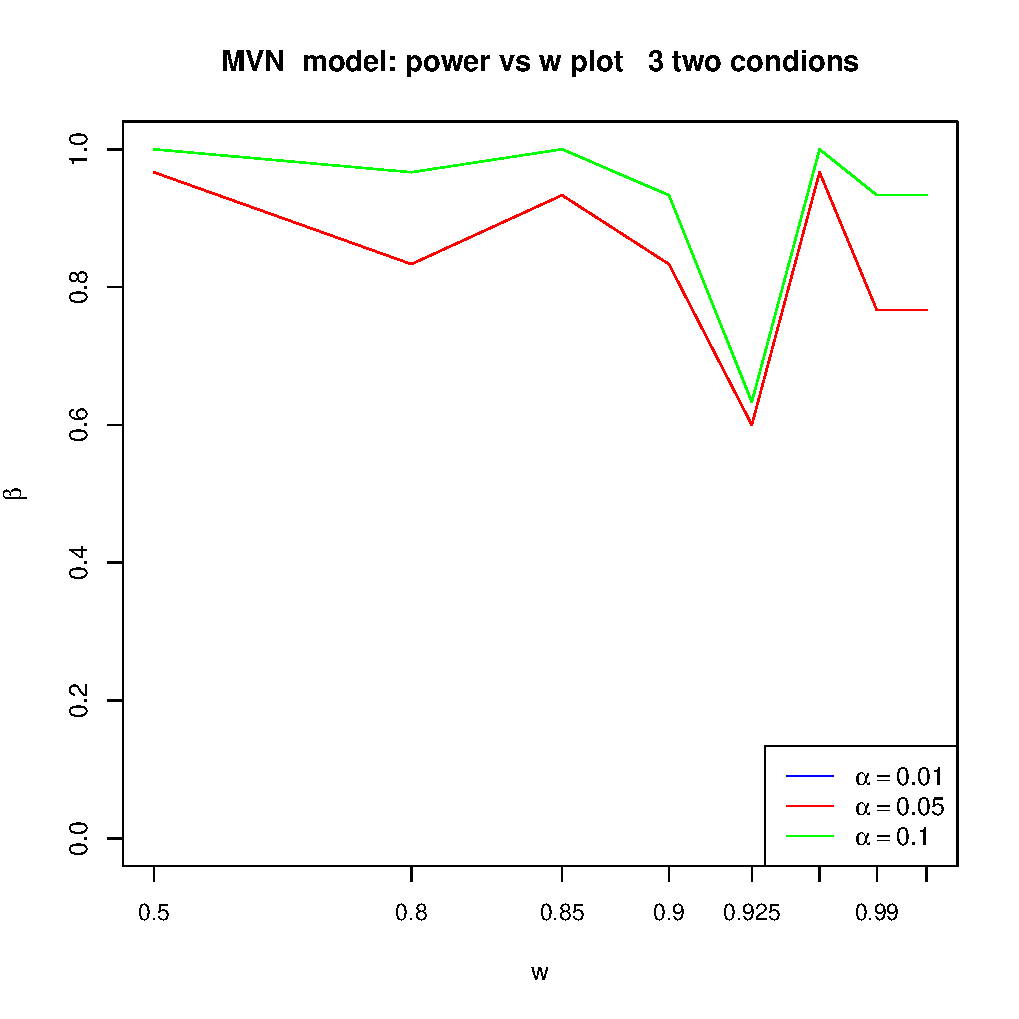
\includegraphics[scale=0.95]{OOSMVN-power-w-c0-01-3-cond.pdf}
\caption{Power ($\beta$) vs Type I error ($\alpha$) plot for different $w$ values for the Gaussian setting (noisy case)}
\label{fig:MVN-c001-power-w-Kcond}
\end{figure}

\section{Experiments on Wiki Data}
To test the JOFC approach with real data, a collection of articles are collected from the English Wikipedia, consisting of the
 directed 2-neighborhood of the document "Algebraic Geometry". 
   This  collection of 1382 articles and the correspondence of each article in French 
Wikipedia is our real-life dataset. It is possible to utilize both textual content of the documents and the hyperlink graph structure. The textual content of the documents is summarized by the bag-of-words model. Dissimilarities between documents  in the same language are computed by the Lin-Pantel discounted mutual information \cite{LinPantel}
 and cosine dissimilarity $k(x_{ik}; x_{jk}) = 1 - (x_{ik} x_{jk})/(\|x_{ik}\|_2\|x_{ik}\|_2)$. 
 The dissimilarities based on the hyperlink graph of the collection of the articles are 
 for each pair of vertices $i$ and $j$, the number of vertices one must travel to go from $i$ to $j$.   
We will only consider dissimilarities based on the textual content in this example.
   
Our exploitation task is still testing for matchedness of vertices between different conditions, in this case wiki articles from different languages.
For hypothesis testing,   randomly held out four documents - one matched pair and one unmatched pair
 -  are used to compute empirical type I error $\alpha$ and estimate of power based on the critical value computed
  from the distribution of the test statistic for the remaining 1380 matched pairs. 
The test statistic is computed using one of the three approached mentioned  $cca$, $p\circ m$, and $jofc$ . 
The two sets of held-out matched pairs are embedded as $\tilde{y}_1$ and $\tilde{y}_2$, via out-of-sample
embedding, to estimate the null distribution of the test statistic $T = d(\tilde{y}_1; \tilde{y}_2)$. This allows
us to estimate critical values for any specified Type I error level. 
Then the two sets of heldout unmatched pairs are embedded as $\tilde{y'}_1$ and $\tilde{y'}_2$, via out-of-sample embedding. 
$T' = d(\tilde{y'}_1; \tilde{y'}_2)$ will give us an empirical distribution of the test statistic  under the alternative hypothesis. 
And the distribution under null hypothesis and under alternative hypothesis can be used to estimate power.
Target dimensionality d is determined by the Zhu and Ghodsi  automatic dimensionality selection
method \cite{ZhuGhodsi}, resulting in d = 6 for this data set.



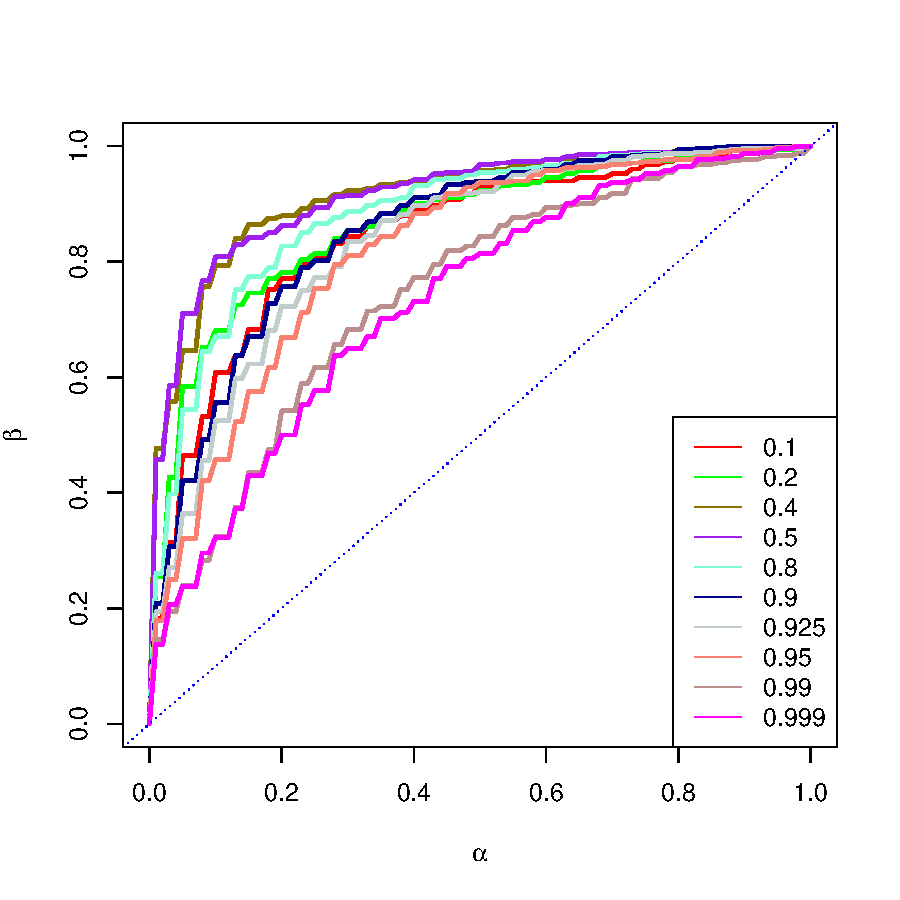
\includegraphics{FidCommPaper-wiki-2cond-plot}


\section{Model Selection}
For the simulations presented up to now, the embedding dimension $d$  was set to 2. This was a convenient choice which allowed us to investigate various aspects of JOFC and competing approaches.
However we require more care in selection of this parameter, since it plays such a big role in performance in general learning settings. Specifically, we want to consider the effect of this parameter on Fidelity and Commensurability.
First consider the distribution of the test statistic for different values of the embedding dimension in the Gaussian setting.


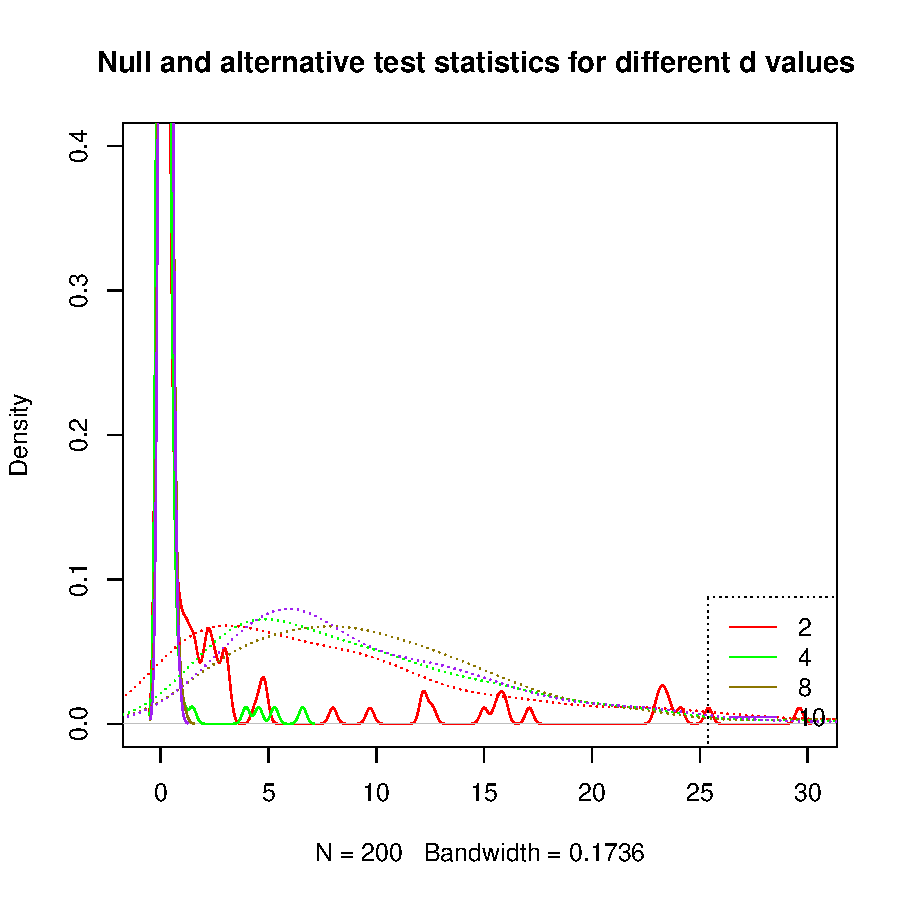
\includegraphics{FidCommPaper-fig-stats-d}
The plot here shows the effect of $d$ on Fidelity and Commensurability errors.
 


\section{Experiments on Graph Data}

We wish to apply our approach to  the vertex matching problem in multiple graphs. These simulations will be for the same semi-supervised setting as mentioned in \ref{sec:RelatedWork}, where matchings between some vertices in different graphs are known 
  and the task is to infer the correspondences between the remaining collection of vertices in the graphs.

Suppose $A,B \in \mathcal{R}^{(r+s)\times (r+s)}$ are adjacency matrices for graphs 
 partitioned as ($r$ rows then $s$ rows, $r$ columns then $s$ columns)
\[  A =\left [
\begin{array}{cc} A_{11} & A_{12} \\ A_{21} & A_{22} \end{array} \right ]
\ \ \ \ \ \ \ \ \ B =\left [
\begin{array}{cc} B_{11} & B_{12} \\ B_{21} & B_{22} \end{array} \right ]
\]
To simplify  suppose that $A_{11}=B_{11}$ , ie the first $r$ vertices
of $A$'s graph correspond respectively to the first $r$ vertices of $B$'s graph,
and we wish to complete the isomorphism by determining the correspondences between the pairs of $s$ vertices. 
That is, we seek a permutation matrix $P \in \{0,1\}^{s \times s}$ such that $A=(I_{r \times r}
\oplus P)B(I_{r \times r} \oplus P)^T$, ie
 \[
 \left [
\begin{array}{cc} A_{11} & A_{12} \\ A_{21} & A_{22} \end{array}
\right ]
\left [
\begin{array}{cc} I_{r \times r} & 0_{r \times s} \\ 0_{s \times r} & P \end{array}
\right ]
=
\left [
\begin{array}{cc} I_{r \times r} & 0_{r \times s} \\ 0_{s \times r} & P \end{array}
\right ]
\left [
\begin{array}{cc} B_{11} & B_{12} \\ B_{21} & B_{22} \end{array}
\right ] .
\]

Using omnibus  embedding, it is possible to embed the vertices of two graphs in a commensurate space.
Therefore, the JOFC approach can be used here for determining the pairwise distances between  the vertices of $A$ and $B$.
The next step is to use the pairwise distances to find the optimal 1-1 matchings by the Hungarian algorithm \cite{Hung-algo}. The Hungarian algorithm finds an optimal matching between two sets of vertices such that the total  cost which is the sum of the pairwise distances of matched nodes is minimized.
 
One useful property of dissimilarity representation is that the structure of data is irrelevant once an appropriate dissimilarity function  for the data is available. 
There are many distances that can be defined between vertices in graphs. We assume that an appropriate distance measure is available to us.
In our experiments we will use three different dissimilarities between vertices in a graph:
\begin{itemize}
 \item the shortest path on the  unweighted graph whose adjacency matrix is available
 \item the shortest path on a weighted version of the graph whose adjacency matrix is available
 \item diffusion distance between vertices on the (unweighted) graph.
 \end{itemize}
 We will omit the results for weighted graph dissimilarities, since they seem to have the same performance as the weighted dissimilarities.
 
 Note that these dissimilarities can only be defined between vertices of the same graph. We impute the inter-condition dissimilarities   as described before\ref{omnibus}.
 
  In the following simulation, $A$ is the adjacency matrix of an Erdos-Renyi graph, that is
  $\left[A\right]_{ij} \sim Binomial(p)$ where $\left[A\right]_{ij}$ is $ij$-th entry of the adjacency matrix  $A$.
   and the adjacency matrix  $B$ is a entry-wise bit-flipped version of the adjacency matrix of $A$, that is
   In the following simulation, $A$ is the adjacency matrix of an Erdos-Renyi graph, that is
  $\left[A\right]_{ij} \sim Binomial(p)$ where $\left[A\right]_{ij}$ is $ij$-th entry of the adjacency matrix  $A$.
   and the adjacency matrix  $B$ is a entry-wise bit-flipped version of the adjacency matrix of $A$, that is
   $\left[B\right]_{ij}|\left[A\right]_{ij}=0 \sim Binomial(p_{10})$ $\left[B\right]_{ij}|\left[A\right]_{ij}=1 \sim Binomial(p_{11})$. Suppose $p_{10}=p_{11}=p$.
  
  The probability of flipping an entry of the adjacency matrix is the perturbation parameter $p_{pert}$ which is the variable on the x-axis. 
  The performance measure is the proportion of true matches to the number of matches. Note that 
  under chance the expected number of true matches is 1, as shown with the dashed line. In the simulation, $r=20$ and $s=5$. $p_{pert}$ varies from $0$ to $1$ in increments of $0.1$. 
\begin{figure}
  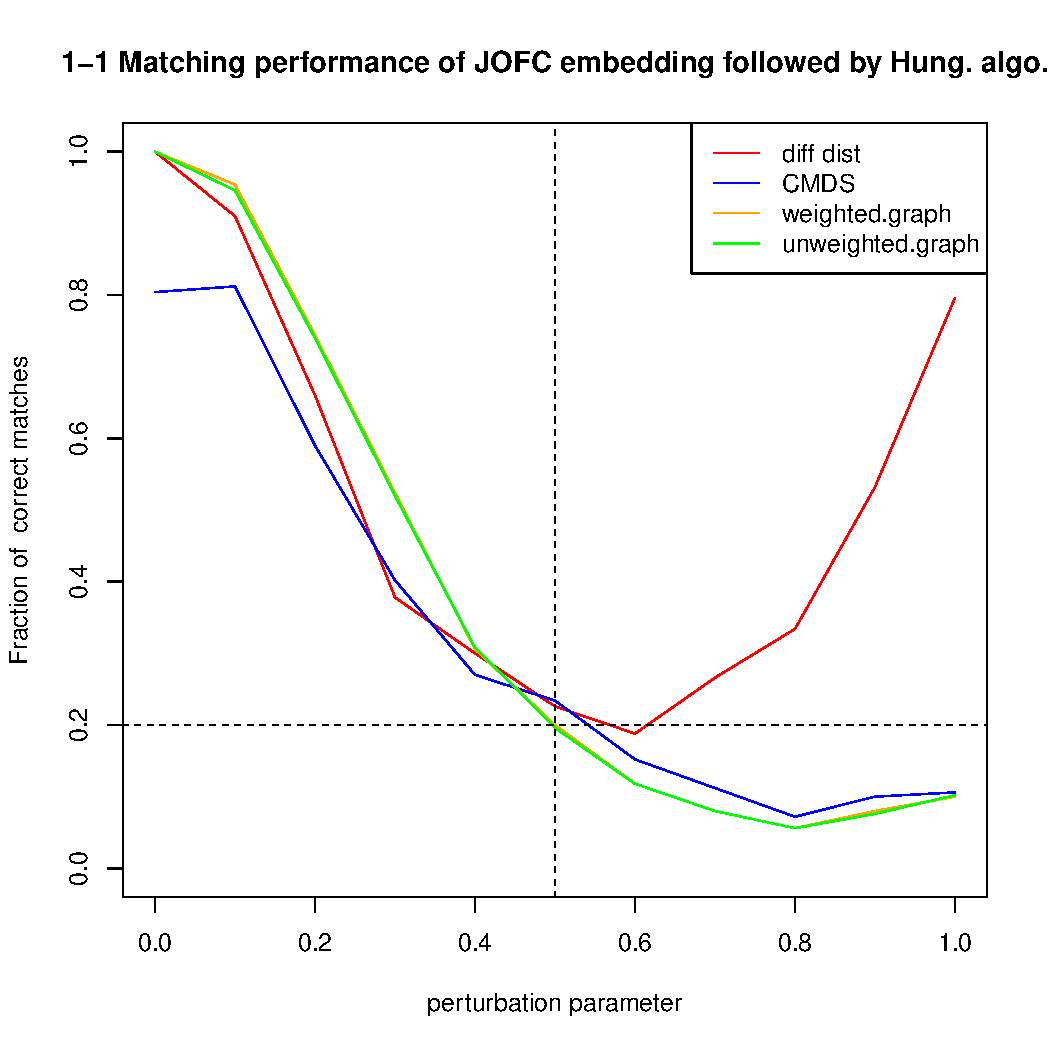
\includegraphics[scale=0.65]{FidCommPapergraph-plot-1.pdf}
\end{figure}


In the plot above, JOFC approach applied to  dissimilarities based on weighted and unweighted graphs is compared with classical MDS on dissimilarities of weighted graphs.

Note that JOFC for unweighted and weighted graphs  have better performance compared to CMDS. As the perturbation parameter gets larger, the performance degrades until it is indistinguishable from random chance at $pert=0.5$.

Another feature of the plot is the U-shape of the curve for diffusion-distance based dissimilarities. This invariancy with respect to complement of the graph should be investigated further.

An interesting trend in the graph is that shortest-path based dissimilarities are an improvement over diffusion-path dissimilarities for perturbation parameter less than 0.5 , but as perturbation parameter increases past 0.5, fraction of correct matches for diffusion distance based dissimilarity recovers, while for other dissimilarities the fraction continues to fall. 

The dissimilarity type that has the best improvement in performance is JOFC with shortest path distances in weighted graphs(unweighted graphs have similar performance)



This graph shows the effect of the weight parameter of stress $w$ on the probability of true matches.



This graph shows the effect of the diffusion distance parameter $T$ on the probability of true matches for dissimilarities based on diffusion distance.






\section{Conclusion}
 We have investigated the tradeoff between Fidelity and Commensurability and the relation to the weighted raw stress criterion for MDS.
  Two alternative approaches, P$\circ$M and CCA, were presented as extremes of the tradeoff  between Fidelity and Commensurability.
   For  hypothesis testing as the exploitation task, the three approaches were compared in terms of testing power.
    The results indicate that the joint optimization (JOFC) approach is superior to CCA and  P$\circ$M,
     and is also robust to spurious correlations CCA suffers from.
      Also when doing a joint optimization, one should consider an optimal compromise point between Fidelity and Commensurability,
       which corresponds to an optimal weight $w^*$ of the weighted raw stress criterion in contrast to the unweighted raw stress 
        for omnibus matrix embedding. 
        The JOFC approach is quite versatile and can be applied to many problems where data of multiple modalities have to be made commensurate. 
        We have applied JOFC to  test for matches between Wiki articles and pairs of vertices in random graph data.  Performance of JOFC shows that it 
        it is appropriate for these settings.  



\bibliographystyle{plain}
\bibliography{priebe-thesis-JOFC}



\end{document}
